% !TeX program = xelatex
% !TeX encoding = UTF-8
\documentclass[final,5p,twocolumn,10pt]{elsarticle}

\usepackage{amsmath,amssymb,mathtools}
\usepackage{booktabs,multirow,makecell}
\usepackage{graphicx}
\usepackage{xcolor}

% Preserve English sizing and spacing while supporting Chinese filenames/notes.
\usepackage[UTF8,scheme=plain,zihao=false,linespread=1]{ctex}
\setmainfont{Times New Roman}
% Use NewTX's encoded Times family for math operators, retaining the OpenType body font.
\let\PaperTextFamily\rmdefault
\renewcommand{\rmdefault}{ntxtlf}
\usepackage{newtxmath}
\let\rmdefault\PaperTextFamily
% Use one consistent left-aligned display style in the two-column manuscript.
\setlength{\mathindent}{0pt}
\setlength{\jot}{3pt}
\usepackage{placeins}
\usepackage{bicaption}

\usepackage{algorithm}
\usepackage{algpseudocode}
\usepackage{siunitx}
\usepackage{hyperref}
% Keep algorithm line hyperlinks unique when multiple algorithms are present.
\makeatletter
\providecommand{\theHALG@line}{}
\renewcommand{\theHALG@line}{\thealgorithm.\arabic{ALG@line}}
% Align float-only pages at the top instead of stretching gaps vertically.
\setlength{\@fptop}{0pt}
\setlength{\@fpsep}{12pt}
\setlength{\@fpbot}{0pt plus 1fil}
\setlength{\@dblfptop}{0pt}
\setlength{\@dblfpsep}{12pt}
\setlength{\@dblfpbot}{0pt plus 1fil}
\makeatother
\usepackage[nameinlink,capitalise,noabbrev]{cleveref}

\graphicspath{{figures/}}
% Centralize notation here so symbols remain consistent across sections.
\newcommand{\method}{HGNN--PPO}
\newcommand{\R}{\mathbb{R}}
\newcommand{\state}{s_t}
\newcommand{\action}{a_t}
\newcommand{\reward}{r_t}
\newcommand{\policy}{\pi_{\theta}}
\newcommand{\graph}{\mathcal{G}_t}
\newcommand{\nodes}{\mathcal{V}_t}
\newcommand{\edges}{\mathcal{E}_t}
\newcommand{\objective}{J(\theta)}

\DeclareMathOperator*{\argmax}{arg\,max}
\DeclareMathOperator*{\argmin}{arg\,min}


\journal{Target Journal Name}

\begin{document}
\raggedbottom

\begin{frontmatter}

%题目
\title{A Heterogeneous Graph Neural Network and Proximal Policy Optimization Framework for [Problem Name]}


% 作者、单位
\author[aff1]{First Author}
\author[aff1]{Second Author\corref{cor1}}
\ead{corresponding.author@example.com}
\cortext[cor1]{Corresponding author.}
\affiliation[aff1]{organization={Department, University},
  city={City}, postcode={Postcode}, country={Country}}

% 摘要
\begin{abstract}
  Reconfigurable manufacturing systems with auxiliary modules enhance flexibility but complicate resource allocation. 
  Furthermore, traditional scheduling often ignores how post-processing aging treatments affect final product performance. 
  This paper introduces a novel performance-aware flexible job shop scheduling problem with aging-time windows and machine reconfiguration (PFJSP-AW-MR) to simultaneously minimize total weighted tardiness and total performance deviation. 
  First, a mixed-integer linear programming (MILP) model employing piecewise linear fitting is formulated to capture the non-linear temporal evolution of material properties. 
  To solve this strongly NP-hard problem, an improved NSGA-II with a hybrid neighborhood search (INSGA-II\_NS) is proposed. 
  A problem-specific three-layer encoding resolves the spatio-temporal coupling of discrete configurations and continuous aging times. 
  Moreover, a customized two-stage neighborhood search—integrating an improved K-insertion method on an extended disjunctive graph—significantly enhances local exploitation. 
  Extensive benchmark experiments and a real-world industrial case demonstrate that INSGA-II\_NS outperforms well-known multi-objective algorithms, effectively balancing manufacturing performance and production efficiency.

% 配备辅助模块的可重构制造系统增加了资源配置的复杂性，
% 且传统调度常忽视时效处理对产品最终性能的决定性影响。
% 为此，本文提出一类考虑时效时间窗与机器重构的性能感知柔性作业车间调度新问题（PFJSP-AW-MR），
% 旨在同时最小化总加权拖期与总性能偏差。
% 首先，构建混合整数线性规划（MILP）模型，
% 并利用分段线性拟合精确刻画材料属性的非线性时间演化规律。
% 针对该强NP-hard问题，提出一种融合混合邻域搜索的改进NSGA-II算法（INSGA-II\_NS）。
% 其中，定制的三层编码机制有效解决了离散机器配置与连续时效时间之间的时空耦合难题；
% 两阶段邻域搜索算子（结合扩展析取图上的改进K-插入方法）显著增强了算法的局部开发能力。
% 基准算例实验与真实的工业案例研究均表明，
% INSGA-II\_NS在收敛性和多样性上显著优于SPEA2、MOEA/D等先进算法，
% 成功实现了制造性能与生产效率的有效平衡。
\end{abstract}




%关键词
\begin{keyword}
heterogeneous graph neural network \sep proximal policy optimization \sep
deep reinforcement learning \sep scheduling \sep [application keyword]
\end{keyword}

\end{frontmatter}

% 以下Highlights为Elsevier投稿的可选内容；若目标期刊不使用，请删除。
\begin{highlights}
% 依次填写：问题层面的贡献、HGNN表示贡献、PPO决策贡献和最有力的实验结果。
\item [State the problem-level contribution in one sentence.]
\item [State the HGNN representation contribution in one sentence.]
\item [State the PPO decision-making contribution in one sentence.]
\item [State the strongest evidence-based experimental finding.]
\end{highlights}

%【说明】第一章按照应用背景、技术挑战、研究缺口、本文方法、贡献和全文结构展开。
\section{Introduction}
\label{sec:introduction}

Complex products such as aircraft are manufactured through tightly coupled machining and
multi-level assembly processes. Individual parts follow technological routes on shared
resources, while downstream assemblies can start only after all required parts and
subassemblies are available. Scheduling decisions must therefore coordinate resource
competition with synchronization at multiple kitting points. This coordination directly
affects production lead time and the timely delivery of the final product.

%【TODO】补充复杂产品制造装配调度、飞机装配生产组织及齐套约束的已核验参考文献。

The scheduling problem becomes more difficult when the production state changes during
execution. Machine breakdowns temporarily remove capacity, and processing-time variations
alter the completion times of affected operations. A local delay may postpone a downstream
kitting point, block an upper-level assembly, and change the competition for shared
resources. Consequently, the scheduling state is determined by the current resource status
and by the paths through which a disturbance can propagate across technological and
assembly dependencies.

%【说明】本段把本文的动态性限定为机器故障和加工时间波动，不引入尚未建模的紧急插单。
%【TODO】补充机器故障、工时波动及扰动传播相关研究的已核验参考文献。

Existing dynamic scheduling methods commonly rely on dispatching rules, rescheduling
procedures, mathematical programming, or population-based search. These approaches provide
useful mechanisms for reacting to shop-floor changes, but their online use often requires a
trade-off between solution quality and response time. More critically for multi-level
manufacturing-assembly systems, a compact vector of aggregate statistics does not explicitly
retain the heterogeneous relations among operations, resources, components, and assembly
nodes. The loss of this structure makes it difficult to distinguish a local resource delay
from a delay that is likely to propagate through a critical kitting branch.

%【TODO】补充派工规则、反应式重调度、数学规划和元启发式动态调度方法的代表性文献。

Deep reinforcement learning provides an alternative by learning a scheduling policy through
repeated interaction with a simulated environment. Graph neural networks further allow the
policy to operate on scheduling instances with relational structure. However, a homogeneous
or static graph can still merge relations with different scheduling meanings and can leave
event-driven state changes implicit. For the problem considered here, the representation
must distinguish technological precedence, resource eligibility and occupation, component
membership, and multi-level kitting. It must also update these relations and their features
after each observed event without exposing future disturbances to the policy.

%【TODO】补充图神经网络调度、异构图表示及深度强化学习动态调度的已核验文献。

This study develops a disturbance-aware dynamic HGNN-PPO method for event-driven
multi-level manufacturing-assembly scheduling. A discrete-event simulator first records
operation progress, resource availability, realized processing times, and kitting readiness.
At each decision epoch, these records are converted into a typed heterogeneous graph. A
multi-relation heterogeneous graph neural network (HGNN) propagates and fuses information
according to relation semantics, and proximal policy optimization (PPO) learns a scheduling
policy from the resulting graph representation \cite{schulman2017ppo}. The method thereby
connects the physical event process, the structural paths of disturbance propagation, and
the executable scheduling decision within one closed loop.

%【说明】核心术语统一为dynamic multi-level manufacturing-assembly scheduling、dynamic heterogeneous graph、HGNN和PPO。

The contributions of this study are summarized as follows.

\begin{itemize}
  \item A dynamic multi-level manufacturing-assembly scheduling formulation is established
  for machine breakdowns and processing-time variations. The formulation separates
  immutable execution history from adjustable operations and embeds technological,
  resource, and kitting constraints in a common event-driven environment.

  \item A disturbance-aware dynamic heterogeneous graph is constructed to represent
  manufacturing operations, assembly operations, assembly objects, and resources. Typed
  relations preserve the routes along which local disturbances affect shared capacity and
  downstream kitting conditions.

  \item A multi-relation semantic HGNN-PPO framework is developed to encode the evolving
  graph state and learn an executable scheduling policy. The experimental design evaluates
  parameter settings, component contributions, performance on 30 training instances, and
  generalization on 15 independent test instances.
\end{itemize}

%【TODO】在实验结果全部核验后，重新检查三项贡献中的强度用词，并补充对应的定量证据摘要。
%【TODO】动作空间确定后，将“executable scheduling policy”替换为精确的动作定义。

The remainder of this paper is organized as follows. Section~\ref{sec:literature} reviews
dynamic scheduling, deep reinforcement learning, and graph-based scheduling methods.
Section~\ref{sec:problem} defines the scheduling problem, mathematical formulation, and
discrete-event environment. Section~\ref{sec:method} presents the dynamic heterogeneous
graph, the multi-relation HGNN encoder, and the PPO policy. Section~\ref{sec:experiments}
reports the experimental dataset, parameter setting, ablation experiment, comparative
results, and generalization analysis. The final section concludes the study and outlines
directions for further work.

%【说明】第二章按照方法类别组织相关工作，每一节均以与本文直接相关的研究缺口收束。
\section{Literature Review}
\label{sec:literature}

\subsection{Dynamic Scheduling in Manufacturing Systems}
\label{subsec:traditional_methods}

Dynamic scheduling methods differ mainly in when they react to an event and how they
construct the revised schedule. Reactive dispatching rules select an operation or resource
from the currently feasible set and therefore provide short decision times. Predictive-
reactive methods start from a baseline schedule and repair or regenerate it after a
disturbance. Mathematical programming and metaheuristic methods can explore a wider solution
space, whereas rolling-horizon and event-driven mechanisms restrict each optimization to the
information available at the current time.

%【TODO】为派工规则、预测反应式调度、滚动时域、数学规划和元启发式调度分别补充代表性原始文献。

These paradigms provide different balances between responsiveness and search quality.
Dispatching rules are inexpensive but encode only the information included in their priority
indices. Reoptimization can account for more constraints but may require substantial
computation when disturbances occur frequently. Population-based methods can produce diverse
solutions but repeatedly evaluating candidate schedules can limit their use at dense decision
epochs. The choice of method is therefore inseparable from the state representation and the
time available for online decisions.

Multi-level manufacturing-assembly systems introduce an additional coordination requirement.
A manufacturing delay changes not only the completion time of one route but also the release
time of an assembly that waits for several branches. Shared resources couple otherwise
separate routes, and successive kitting points propagate the effect toward higher assembly
levels. Existing dynamic scheduling formulations do not automatically preserve these paths
when the system is summarized by global workload and utilization indicators. This motivates
a relational representation that remains synchronized with the event-driven environment.

%【TODO】补充多级装配、齐套调度和制造装配协同调度的已核验文献，并明确本文问题与柔性作业车间调度的区别。

\subsection{Deep Reinforcement Learning for Dynamic Scheduling}
\label{subsec:drl_scheduling}

Deep reinforcement learning formulates scheduling as sequential interaction among a state,
an action, a transition mechanism, and a reward. Value-based methods estimate the long-term
return of discrete decisions, while policy-gradient and actor-critic methods optimize a
parameterized policy directly. Once trained, these approaches can produce decisions through
network inference and are therefore attractive for event-driven environments that require
repeated online responses.

%【TODO】补充价值型、策略梯度型和Actor-Critic调度方法的代表性原始文献。

The performance of a learned scheduler depends on how the Markov decision process is
constructed. State variables must expose information needed to distinguish feasible and
consequential actions. The action space must correspond to decisions that the simulator can
execute, and feasibility masking must prevent violations of precedence, kitting, and resource
capacity. The reward must remain aligned with the reported scheduling objectives. A policy
can otherwise converge in its training environment while optimizing a surrogate that does
not correspond to the final evaluation.

Generalization is another central issue. A policy trained on a limited set of instances may
associate decisions with a fixed number or ordering of operations. Relational encoders,
parameter sharing, randomized training scenarios, and independent test instances have been
used to reduce this dependence. Nevertheless, generalization claims require an explicit
train-test boundary and a precise description of what changes between the two partitions.
This requirement is particularly important when topology, scale, and disturbance intensity
can vary independently.

%【TODO】补充调度策略泛化、可行性掩码、奖励设计和独立测试协议方面的已核验文献。

\subsection{Graph Representation Learning for Scheduling}
\label{subsec:graph_scheduling}

Graph-based scheduling methods encode operations and resources as nodes and express
precedence or eligibility through edges. Message passing aggregates information from local
neighborhoods, which supports variable-size instances and preserves structural constraints
more directly than a fixed-length state vector. Attention mechanisms can further assign
different weights to neighboring entities when their current influence on a decision differs.

Homogeneous graphs use a shared transformation for all nodes or edges. This representation is
effective when the encoded relations have similar meanings, but manufacturing-assembly
scheduling contains several distinct semantics. A technological edge indicates an execution
order, an eligibility edge indicates a possible resource assignment, an occupation edge
records a current physical state, and a kitting edge synchronizes multiple branches. Treating
these relations identically can obscure why information from a neighbor should influence the
current operation.

Heterogeneous graph neural networks address this issue by using type-specific projections and
relation-specific message functions. For dynamic scheduling, the graph must additionally
distinguish persistent production structure from event-dependent features. An effective model
should update the affected portion of the graph after an event, retain the semantic identity
of each relation, and provide a graph-level representation for policy learning. These needs
motivate the dynamic heterogeneous representation and multi-relation semantic encoder used in
this study.

%【TODO】补充图调度、图注意力、异构图神经网络及动态图学习的代表性原始文献。

\subsection{Research Gaps and Motivation}
\label{subsec:graph_drl}

The literature indicates three connected gaps. First, common dynamic scheduling states do not
explicitly preserve the propagation of a local event through shared resources and successive
kitting levels. Second, graph-based schedulers often emphasize technological precedence and
resource eligibility but do not distinguish all relations required by multi-level assembly.
Third, experimental generalization is sometimes inferred from training performance without a
strictly separated test partition or a clear definition of the distribution shift.

The present study addresses these gaps through a common environment-representation-policy
interface. The discrete-event simulator defines how disturbances change physical feasibility.
The dynamic heterogeneous graph records both persistent structure and current event effects.
The multi-relation HGNN preserves semantic differences during message propagation, and PPO
optimizes the policy over the resulting state. The experiment design separates 30 training
instances from 15 independent test instances so that training behavior and transfer behavior
can be discussed independently.

%【TODO】完成文献检索后增加相关工作对比表，至少比较问题类型、扰动类型、装配关系、图类型、决策方法和泛化设置。
%【TODO】当前参考文献库仅含PPO条目，投稿前必须补齐本章所有文献并逐条核验DOI、作者、年份和方法归属。

% 第三章精简稿：引用已有静态模型，仅展开动态扩展、双目标与执行环境。
\section{Problem Description and Mathematical Formulation}
\label{sec:problem}

\subsection{Problem Description}
\label{subsec:problem_description}

This study extends the flexible job shop scheduling problem with multi-level assembly operations
(FJSP-MAOs) of Ning et al.~\cite{ning2027fjspmaos} to dynamic production. Jobs follow prescribed
routes, operations use eligible processing or assembly machines, and compatible jobs can be matched
flexibly to product requirements. Each assembly starts once its required components are ready,
allowing processing and assembly to overlap. The base model supplies technological, machine-capacity,
product-assignment, and assembly-matching constraints.

% 沿用Ning等的工艺、资源及柔性装配模型，保留分级齐套与加工装配并行。
% 不再重复推导已有静态约束，后文仅定义动态执行所需的扩展。

Figure~\ref{fig:problem_description} illustrates three disturbances: processing-time variations change
operation durations, machine failures interrupt capacity and possibly running work, and urgent arrivals
introduce new jobs and assembly requirements. Their effects propagate through shared machines,
precedence chains, and assembly dependencies. Scheduling uses only revealed information and adjusts
unstarted or interrupted work while preserving completed records and unaffected execution. The
objectives are makespan and deviation from the initial baseline plan.

% 三类事件分别改变工时、机器可用性与任务集合，其影响沿资源和装配依赖传播。
% 冻结已完成记录及正常在制安排，只调整等待或中断任务，并兼顾效率与稳定性。

\begin{figure*}[t]
 \centering
 \captionsetup{name=Figure}
 \includegraphics[width=0.9\textwidth]{figures/F1动态加工-装配调度场景图.png}
 \caption{Dynamic processing--assembly scheduling under duration changes, failures, and urgent arrivals.}
 \label{fig:problem_description}
\end{figure*}

\subsection{Reactive Scheduling Model}
\label{subsec:mathematical_model}

Let $S^0$ be the baseline for initial operation set $\mathcal O^0$, with start times $B^0_{ij}$,
machine assignments $X^0_{ijk}$, and makespan $C^0_{\max}>0$. At time $t$, admitted operations are
$\mathcal O(t)=\mathcal O^0\cup\mathcal O^{\mathrm{new}}(t)$, where the second set contains arrived
urgent orders. Waiting and failure-interrupted operations form the adjustable set
\begin{equation}
 \mathcal O^R(t)=\mathcal O^{\mathrm{wait}}(t)\cup\mathcal O^{\mathrm{int}}(t).
 \label{eq:adjustable_operations}
\end{equation}
Variables $B_{ij},E_{ij}$ describe the next successful execution attempt; interrupted attempts remain
in the log. Binary variables $X_{ijk}$ and $Y_{iji'j'}$ encode assignment and machine order.
For eligible machines $K_{ij}$, current durations are
$\widetilde{pt}_{ijk}(t)=pt_{ijk}[1+\varepsilon_{ij}(t)]$, with $\varepsilon_{ij}(t)>-1$.

% 基准计划只覆盖原订单；插单到达后扩展工序集合。B和E表示成功执行段，
% 中断历史仍保留。工时波动只使用当前已观测信息。

The two objectives are
\begin{equation}
 \begin{aligned}
 \min\ f_1(S)&=C_{\max},\\
 \min\ f_2(S)&=D_{\mathrm{dev}}(S,S^0),
 \end{aligned}
 \label{eq:scheduling_objectives}
\end{equation}
with normalized deviation
\begin{equation}
 \begin{aligned}
 D_{\mathrm{dev}}(S,S^0)
 &=\frac{\lambda_B}{|\mathcal O^0|C^0_{\max}}
 \sum_{O_{ij}\in\mathcal O^0}|B_{ij}-B^0_{ij}|\\
 &\quad+\frac{\lambda_X}{2|\mathcal O^0|}
 \sum_{O_{ij}\in\mathcal O^0}\sum_{k\in K_{ij}}|X_{ijk}-X^0_{ijk}|.
 \end{aligned}
 \label{eq:objective_deviation}
\end{equation}
where $\lambda_B,\lambda_X\ge0$ and $\lambda_B+\lambda_X=1$. Deviation measures start-time changes
and reassignment of baseline operations; the factor two accounts for the two assignment entries
changed by a machine switch. Urgent orders contribute to makespan but have no baseline deviation.

% 双目标保留原定义；插单没有基准记录，不计偏离度，但必须计入工期。

For $O_{ij}\in\mathcal O^R(t)$, assignment, completion, and release constraints are
\begin{equation}
 \begin{aligned}
 \sum_{k\in K_{ij}}X_{ijk}&=1, \\
 E_{ij}&=B_{ij}+\sum_{k\in K_{ij}}X_{ijk}\widetilde{pt}_{ijk}(t),
 \\
 B_{ij}&\ge\max\{t,r_i\}, \\
 C_{\max}&\ge E_{ij},\quad O_{ij}\in\mathcal O(t).
 \end{aligned}
 \label{eq:execution_constraints}
\end{equation}
Here $r_i$ is no earlier than the arrival of its order. Technological and assembly predecessor sets
$\mathcal P^{\mathrm{pro}}_{ij}$ and $\mathcal P^{\mathrm{asm}}_{ij}$ impose
\begin{equation}
 \begin{aligned}
 B_{ij}&\ge E_{i'j'}, &&O_{i'j'}\in\mathcal P^{\mathrm{pro}}_{ij},
 \\
 B_{ij}&\ge E_{i'j'}, &&O_{i'j'}\in\mathcal P^{\mathrm{asm}}_{ij},
 \\
 B_{ij}&\ge\sum_{k\in K_{ij}}X_{ijk}t_k^{\mathrm{ava}}(t).
 \end{aligned}
 \label{eq:precedence_constraints}
\end{equation}
Machine availability $t_k^{\mathrm{ava}}(t)$ includes running work and known repair intervals;
machines with unknown recovery times remain unavailable until recovery. Assembly predecessors follow
the selected feasible matching. Completed assemblies and committed component usage cannot be undone.

% 保留资源分配、释放、前驱和可用时间约束。装配前驱随合法匹配确定，
% 不提前固定所有工件归属；已完成装配及已投入组成件不可撤销。

For an interrupted operation, let $k^f_{ij}$ be its failed machine. Waiting for repair
($u^{\mathrm{rec}}_{ij}=0$) or rerouting ($u^{\mathrm{rec}}_{ij}=1$) satisfies
\begin{equation}
 \begin{aligned}
 X_{ij k^f_{ij}}&=1-u^{\mathrm{rec}}_{ij}, \\
 \sum_{k\in K_{ij}\setminus\{k^f_{ij}\}}X_{ijk}&=u^{\mathrm{rec}}_{ij}.
 \end{aligned}
 \label{eq:recovery_constraints}
\end{equation}
Both alternatives restart the operation with its updated full duration. An empty alternative-machine
set forces waiting. Records representing one joint assembly share the same recovery decision.

% 故障工序可等待或改派，均按完整工时重新加工；联合装配一致恢复。

For distinct adjustable execution activities and $k\in K_{ij}\cap K_{i'j'}$, non-overlap requires
\begin{equation}
 \begin{aligned}
 B_{i'j'}&\ge E_{ij}-M(1-Y_{iji'j'})
 -M(2-X_{ijk}-X_{i'j'k}), \\
 B_{ij}&\ge E_{i'j'}-MY_{iji'j'}
 -M(2-X_{ijk}-X_{i'j'k}),
 \end{aligned}
 \label{eq:machine_capacity}
\end{equation}
with sufficiently large $M$. Component records of the same physical assembly instead obey the
inherited synchronization constraints. Completed records are fixed; unaffected running operations retain
their assignments and start times. Their completion estimates change only with observed duration
updates. All time variables are nonnegative and assignment, order, and recovery variables are binary.

% 同机互斥针对不同物理活动，不排斥同一次联合装配的同步记录。
% 冻结执行历史，保留变量域与已观测信息边界。
% TODO：基准生成、权重、扰动分布及随机种子仍须在实验设置中核验。

\subsection{Event-driven Discrete-event Simulation Environment}
\label{subsec:dynamic_environment}

The simulator takes an initial instance, baseline $S^0$, finite scenario $\Xi$, and scheduling
policy $\pi$. Its internal state $\mathcal X$ records operation status, timing, assignments, machine
availability, assembly commitments, and an event calendar. Completion, failure, recovery, duration
updates, and order arrivals induce event transitions; executable scheduling decisions induce decision
transitions:
\begin{equation}
 \begin{aligned}
 \mathcal X(t^+)&=\mathcal T_{\mathrm{evt}}(\mathcal X(t^-),\mathcal E(t)),\\
 \mathcal X_{n+1}&=\mathcal T_{\mathrm{dec}}(\mathcal X_n,d_n).
 \end{aligned}
 \label{eq:event_decision_transition}
\end{equation}
The observation $x_n$ excludes unrevealed future events. At a shared timestamp, completion precedes
failure, followed by recovery, duration updates, and arrivals. Failure cancels the interrupted
attempt's completion event; a duration change replaces the affected completion prediction without
scheduling an event in the past. Arrivals add tasks and their assembly requirements.

% 仿真仅保留事件转移与决策转移的统一接口，删除与伪代码重复的展开公式。
% 同刻先完成后故障，再处理恢复、工时更新与插单；未来事件不向策略泄露。

Algorithm~\ref{alg:reactive_simulation} repeatedly executes decisions from the current feasible set
$\mathcal D_n$. When no decision remains, time advances to the next event. Feasibility includes
machine capacity, predecessor readiness, and assembly matching. The episode ends only after all orders
in the finite scenario have arrived and completed; unfinished work with an empty calendar is reported
as infeasible. Outputs are the execution log, makespan, and baseline deviation.

% 无可行决策才推进时间；存在后续插单时不提前结束，空队列未完工报告不可行。

\begin{algorithm}[t]
\caption{Event-driven reactive scheduling}
\label{alg:reactive_simulation}
\small
\begin{algorithmic}[1]
\Require Instance, baseline $S^0$, scenario $\Xi$, policy $\pi$
\Ensure $S$, $C_{\max}(S)$, $D_{\mathrm{dev}}(S,S^0)$
\State Set $t\gets0$, $n\gets0$; initialize state and events
\While{unfinished work or future arrivals remain}
 \State Process current events; update state
 \State Construct feasible set $\mathcal D_n$
 \While{$\mathcal D_n\ne\varnothing$}
  \State Select $d_n\gets\pi(x_n,S^0,\mathcal D_n)$
  \State Execute $d_n$; update state and events
  \State $n\gets n+1$; recompute $\mathcal D_n$
 \EndWhile
 \If{unfinished work or future arrivals remain}
  \If{the event calendar is empty}
   \State Report infeasibility and stop
  \EndIf
  \State Advance time to the next event
 \EndIf
\EndWhile
\State \Return $S$, $C_{\max}(S)$, $D_{\mathrm{dev}}(S,S^0)$
\end{algorithmic}
\end{algorithm}

% 第四章采用大论文的状态编码与三头规则选择框架。
% 英文进入正文；中文仅作核对与待补充说明，不参与排版。
\section{Dynamic Heterogeneous Graph-based Rule Selection}
\label{sec:method}

Dynamic processing--assembly scheduling requires a policy to distinguish changes in operation progress,
resource availability, and assembly readiness. These changes have different implications for routing,
sequencing, and recovery. The method therefore combines a dynamic heterogeneous graph, meta-path
semantic attention, and decision-specific state readout with three PPO rule-selection heads. The
encoder supplies the state information used to select rules, while the environment enforces the
physical constraints in Section~\ref{sec:problem}.

% 方法区分状态构建、语义编码与策略学习。状态编码为规则选择提供信息，
% 环境继续负责第三章定义的物理约束，不把网络输出直接当成可执行安排。

\subsection{Overall Framework}
\label{subsec:framework_overview}

Figure~\ref{fig:framework} outlines the interaction between the environment and the policy. At
decision index $n$, corresponding to physical time $t_n$, the environment supplies the observation
$x_n$, decision type $\vartheta_n\in\{R,S,RE\}$, and feasible object set
$\mathcal D_n^{\vartheta_n}$. The three types denote machine routing, operation sequencing, and
failure recovery. Several decisions may occur at the same physical time because each dispatch changes
the choices available to subsequent dispatches.

% 环境提供状态、决策类型与可行对象集合。R、S、RE分别对应机器分配、
% 工序排序与故障恢复。同一仿真时刻可以连续执行多个决策。

The observation is mapped to a graph $G_n$. A shared HGNN aggregates typed relations and enhances
node representations through attention over processing--assembly meta-paths. Role-based readout
produces a representation for each decision type. Only the corresponding Actor head is activated to
select a rule from its fixed candidate set. The rule scores feasible objects and returns a concrete
decision to the simulator. Trajectory rewards jointly train the encoder, Actor heads, and Critic.

% 共享编码器先聚合异构关系，再进行元路径注意力增强和角色汇聚。
% 对应Actor头选择规则，规则评价可行对象并生成实际调度决策。

\begin{figure*}[t]
 \centering
 \captionsetup{name=Figure}
 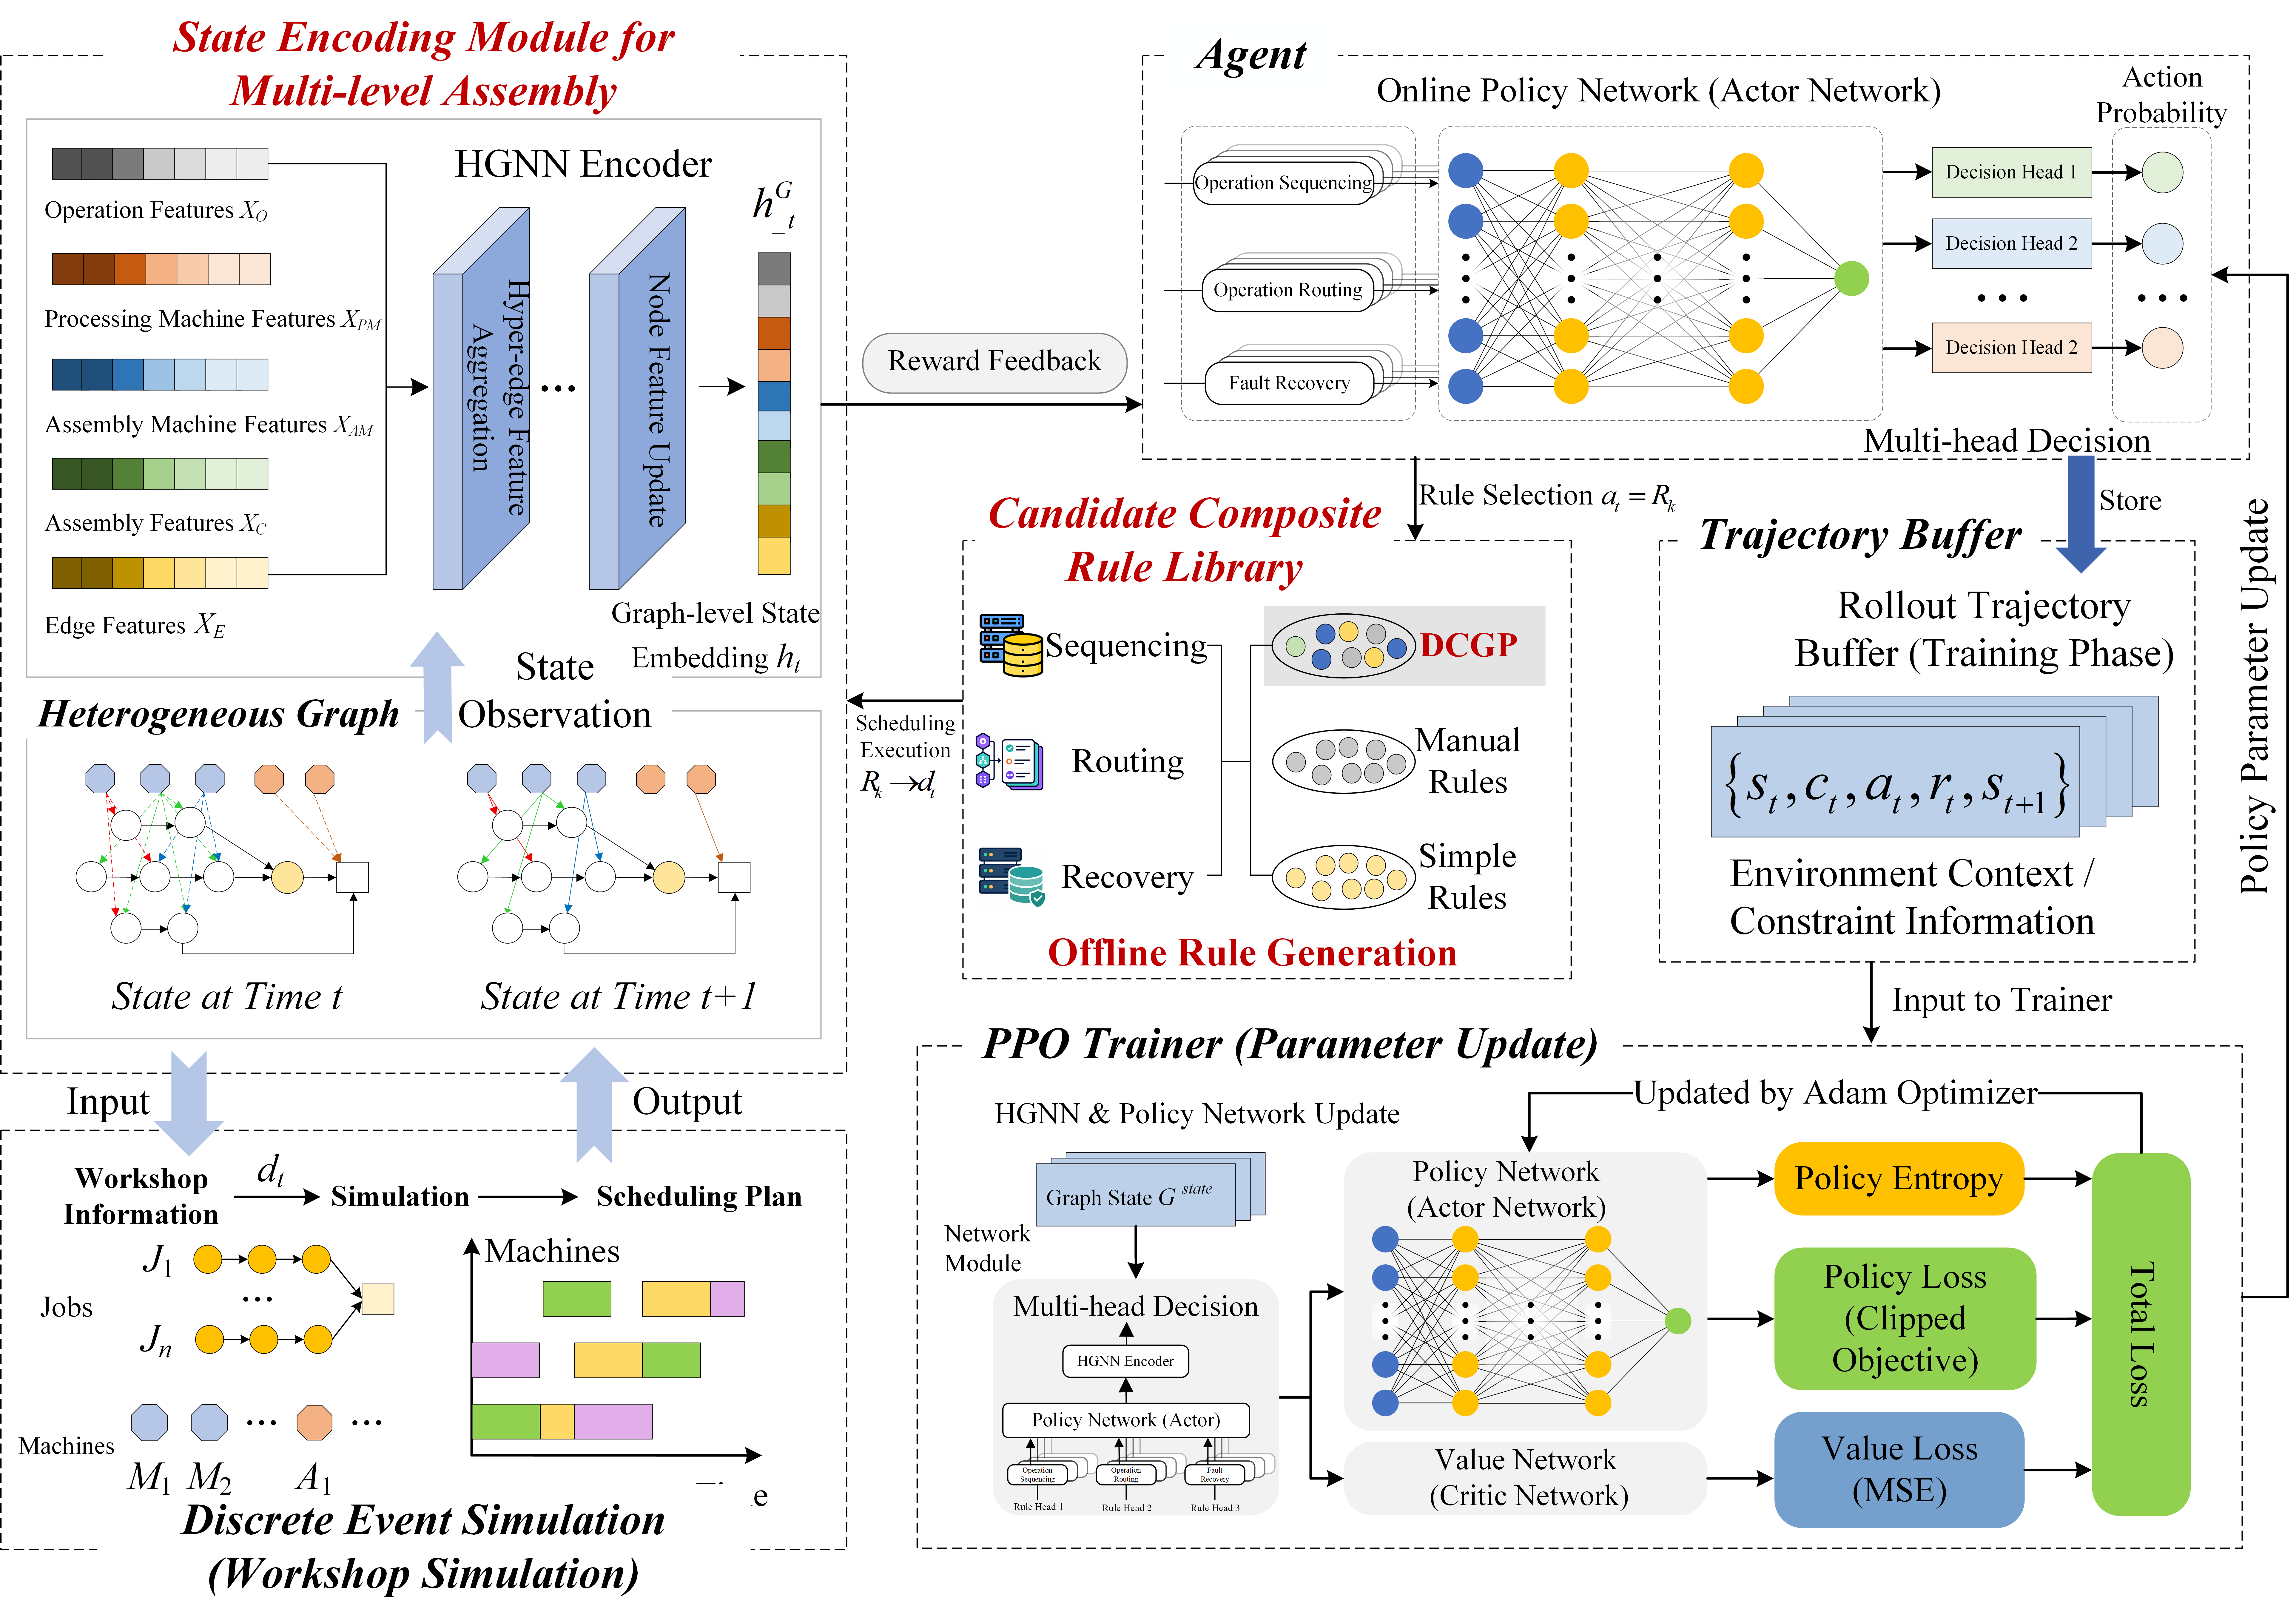
\includegraphics[width=0.95\textwidth]{figures/F2基于规则级决策的反应式调度总体框架.png}
 \caption{Framework of dynamic graph encoding and adaptive dispatching rule selection.}
 \label{fig:framework}
\end{figure*}

A rule action $a_n$ is distinct from the resulting scheduling decision $d_n$. The policy learns which
rule to invoke, rather than directly selecting an operation or machine. Feasibility, including flexible
assembly matching and committed component usage, remains an environment constraint. Candidate rules are
fixed before training and unchanged during evaluation; rule evolution is outside the scope of this
state-encoding method.

% 动作是规则，具体决策是规则调用结果。规则库训练前固定，不展开规则演化。

\subsection{Dynamic Heterogeneous Graph Construction and Update}
\label{subsec:temporal_graph}

\subsubsection{Typed Graph and Observable Features}

The state at decision $n$ is represented as
\begin{equation}
 s_n=(G_n,\boldsymbol{z}_n,\vartheta_n),\qquad
 G_n=(V_n,E_n,\phi,\psi,\boldsymbol{X}_n),
 \label{eq:temporal_graph}
\end{equation}
where $\phi$ and $\psi$ identify node and edge types, $\boldsymbol{X}_n$ contains node features, and
$\boldsymbol{z}_n$ contains observable global statistics. Nodes represent processing operations $O$,
assembly operations $A$, processing and assembly machines $M$, and assembly junctions $S_\ell$.
Start and end nodes delimit the production network. An assembly junction represents a structural
dependency rather than an additional executable task.

% 图中包括加工工序、装配工序、设备和层级装配连接点。
% 起止节点界定生产网络，连接点不额外消耗物理加工资源。

Edges distinguish technological precedence, machine eligibility, active assignments, and assembly
dependencies. Eligibility does not disappear when a machine becomes busy or fails: its current
availability is recorded separately. Undecided assembly matches retain compatible relations, whereas
selected matches are marked as committed. Reverse message-passing relations preserve their semantic
types. This construction retains the flexible matching mechanism of the base problem.

% 候选资格与设备当前可用性分开表示。未确定装配匹配保留兼容关系，
% 实际匹配选定后标记，不提前将所有同类型工件绑定至固定产品。

Operation features describe execution status, release information, current duration estimates,
remaining work, predecessor completion, and baseline deviations. Assembly features describe component
readiness and hierarchy. Machine features describe availability, failure status, occupancy, and load.
An indicator distinguishes operations with baseline records from newly arrived tasks. Global
statistics summarize workload, unfinished tasks, and accumulated deviation. Normalization references
are fixed by the training protocol, without using unrevealed future orders or disturbances.

% 工序、装配与机器分别记录进度、齐套和资源状态；新订单用基准存在标记区分。
% TODO：最终特征清单、缺失值编码和归一化常数须与程序逐项核对。

\subsubsection{Event-driven Graph Update}

The physical transition is defined in Eq.~\eqref{eq:event_decision_transition}; graph updating maps
the resulting state changes into the next observation:
\begin{equation}
 G_{n+1}=\mathcal U_G(G_n,\Delta x_n),
 \label{eq:graph_update}
\end{equation}
where $\Delta x_n$ includes the executed decision and intervening observed events. Assignment activates
an execution relation. Completion releases the machine and updates successor readiness. Failure changes
machine availability and interrupts the affected operation; recovery restores availability. A duration
update revises operation-time and assembly-readiness estimates. An urgent arrival adds its revealed
operations, assembly structure, and machine-eligibility relations.

% 第三章描述物理状态如何变化，本节描述事件如何更新图。
% 完成、故障、恢复、工时波动、插单以及决策执行分别更新相关属性或关系。

Figure~\ref{fig:temporal_graph} illustrates graph evolution during production. Completed nodes may
remain as historical context but cannot be dispatch candidates. Order arrivals can increase graph
size without changing the embedding dimension or the fixed rule-action sets. Dynamic updating here
refers to event-dependent graph structure and features; it does not introduce a recurrent network or
an additional temporal-fusion module.

% 图随插单扩展，编码维数与规则动作数量保持不变。
% 删除原稿额外引入的时序门控，按F3采用当前动态图与执行记录编码。

\begin{figure*}[t]
 \centering
 \captionsetup{name=Figure}
 \includegraphics[width=0.95\textwidth]{figures/F4动态调度过程中的图状态演化.png}
 \caption{Evolution of the heterogeneous scheduling graph during production execution.}
 \label{fig:temporal_graph}
\end{figure*}

\subsection{Meta-path Semantic Attention-based State Encoding}
\label{subsec:hgnn_state}

The encoder in Fig.~\ref{fig:attention_hgnn} distinguishes typed neighborhood aggregation from
semantic fusion. A precedence chain, a shared machine, and an assembly junction convey different
scheduling information even when they connect the same operations. Their representations are therefore
formed separately before attention-based residual enhancement and decision-specific readout.

% 本节是方法重点：关系聚合、元路径语义、注意力残差增强和角色汇聚。

\begin{figure*}[p]
 \centering
 \captionsetup{name=Figure}
 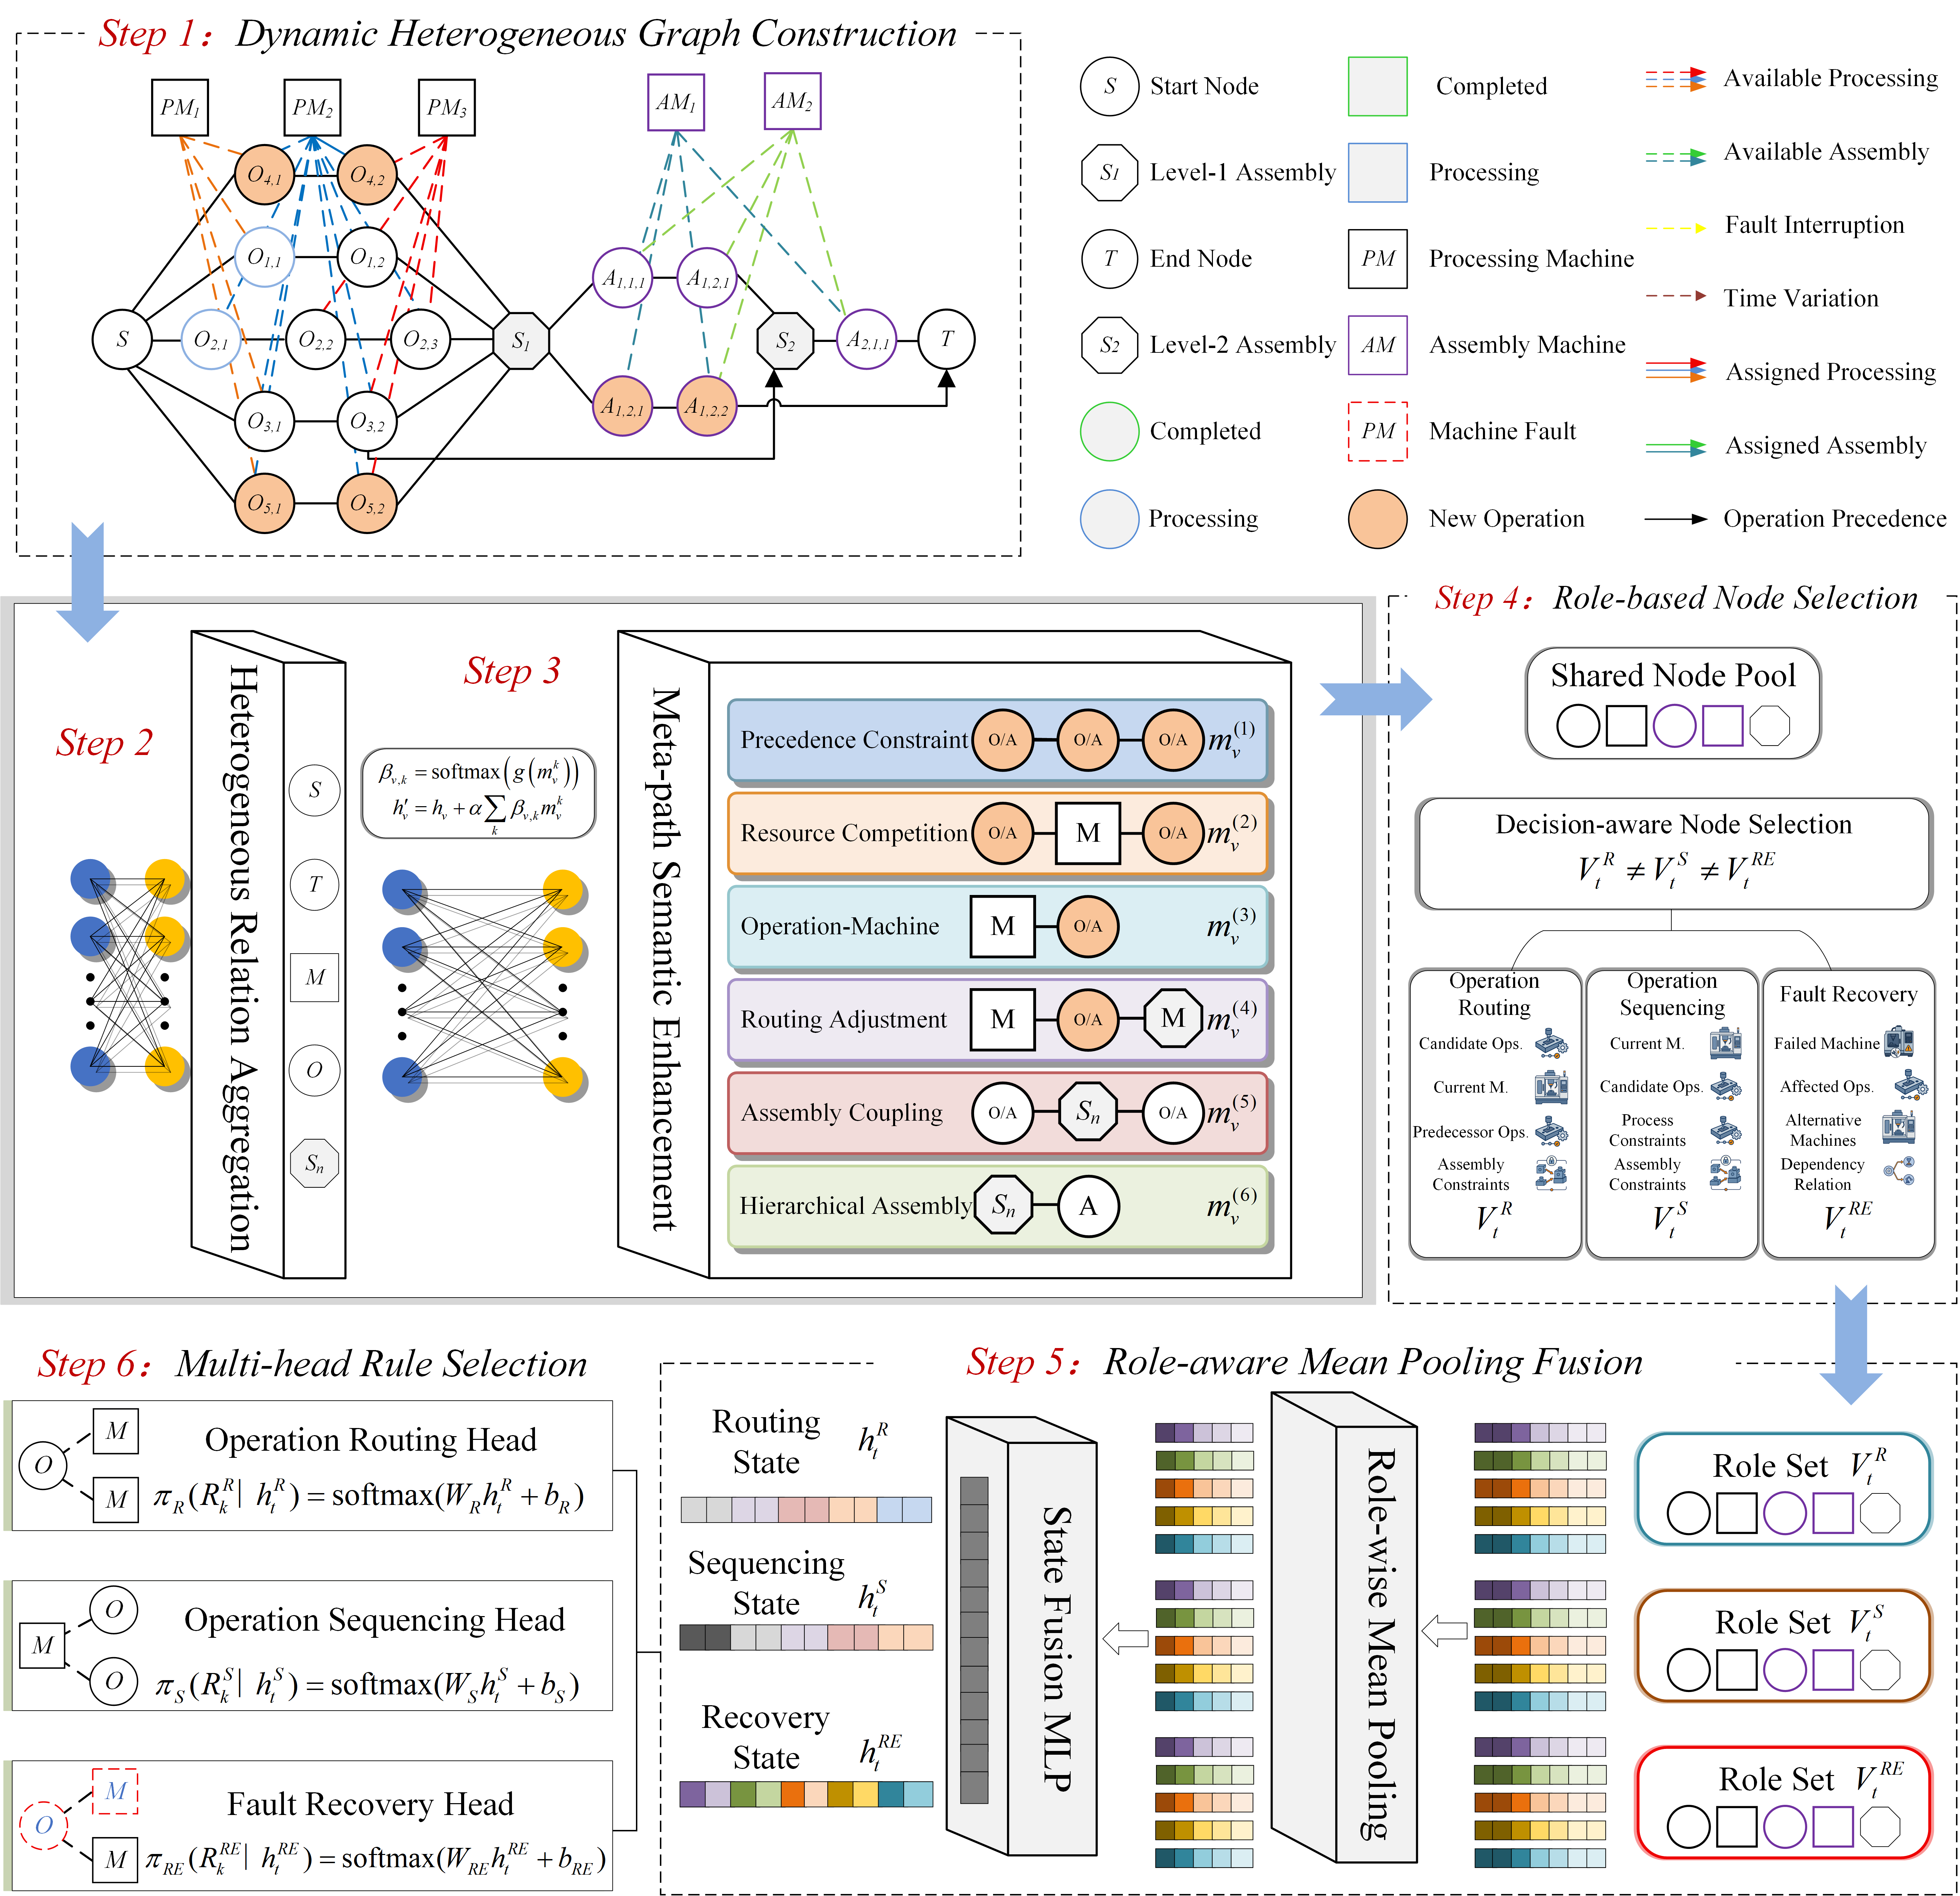
\includegraphics[width=0.98\textwidth,height=0.80\textheight,keepaspectratio]{figures/F3融合装配环境的原路径注意力机制(1).png}
 \caption{Meta-path semantic attention, role-based state readout, and multi-head rule selection.}
 \label{fig:attention_hgnn}
\end{figure*}

\subsubsection{Heterogeneous Relation Aggregation}

Type-specific projections map raw features into a common hidden space:
\begin{equation}
 \boldsymbol{h}^{(0)}_{v,n}
 =\sigma(\boldsymbol{W}_{\phi(v)}\boldsymbol{x}_{v,n}+\boldsymbol{b}_{\phi(v)}).
 \label{eq:type_projection}
\end{equation}
At layer $l$, relation aggregation gives
\begin{equation}
 \boldsymbol{h}^{(l+1)}_{v,n}=\sigma\!\left(
 \boldsymbol{W}_0^{(l)}\boldsymbol{h}^{(l)}_{v,n}
 +\sum_{r\in\mathcal R_G}\sum_{u\in\mathcal N_r(v)}
 \alpha^{(l,r)}_{vu,n}\boldsymbol{W}_r^{(l)}\boldsymbol{h}^{(l)}_{u,n}\right),
 \label{eq:relation_aggregation}
\end{equation}
where $\mathcal N_r(v)$ is the relation-$r$ neighborhood and $\alpha^{(l,r)}_{vu,n}$ denotes
normalized neighbor weights. Each relation has its own mapping, separating machine information from
technological and assembly information. Let $\boldsymbol{h}_{v,n}$ denote the final aggregated embedding.

% 邻居聚合权重与后续语义注意力分属不同层次。
% TODO：核验邻居权重的具体计算、层数、维数及激活函数。

\subsubsection{Processing--Assembly Meta-path Semantics}

Six typed patterns describe complementary scheduling semantics, as listed in
Table~\ref{tab:meta_paths}. Here $O/A$ denotes a processing or assembly operation. The patterns are
computational information paths, not additional physical precedence constraints. For example,
$O/A$--$M$--$O/A$ captures competition through a shared machine, whereas
$O/A$--$S_\ell$--$O/A$ captures coupling through an assembly junction.

% 六类元路径遵循F3，区分工艺、竞争、匹配、路由、装配耦合和层级依赖。

\begin{table}[t]
 \centering
 \captionsetup{name=Table}
 \caption{Meta-path patterns and scheduling semantics.}
 \label{tab:meta_paths}
 \small
 \setlength{\tabcolsep}{3pt}
 \begin{tabular}{@{}c p{0.39\linewidth} p{0.48\linewidth}@{}}
 \toprule
 $k$ & Typed pattern & Scheduling semantics \\
 \midrule
 1 & $O/A$--$O/A$--$O/A$ & Technological and assembly precedence \\
 2 & $O/A$--$M$--$O/A$ & Shared-resource competition \\
 3 & $M$--$O/A$ & Operation--machine association \\
 4 & $M$--$O/A$--$M$ & Routing and reassignment context \\
 5 & $O/A$--$S_\ell$--$O/A$ & Coupling of assembly branches \\
 6 & $S_\ell$--$A$ & Hierarchical assembly dependency \\
 \bottomrule
 \end{tabular}
\end{table}

Let $\mathcal I_k(v,n)$ contain valid instances of pattern $k$ associated with node $v$, and let
$\mathcal N_k(v,n)$ contain their participating nodes. The semantic representation is
\begin{equation}
 \boldsymbol{m}^{(k)}_{v,n}=\operatorname{AGG}_k
 \left(\{\boldsymbol{h}_{u,n}\}_{u\in\mathcal N_k(v,n)}\right).
 \label{eq:meta_path_embedding}
\end{equation}
The pattern-specific operator retains semantic identity when aggregating participating nodes.
Absent patterns are excluded from attention normalization. Thus a missing assembly branch or an
inapplicable routing pattern is not interpreted as an informative zero-valued observation.

% AGG是对F3路径聚合模块的接口表达，不虚构尚未核验的具体实现。
% TODO：核验路径实例、方向、重复计数及AGG算子，补齐可复现定义。

\subsubsection{Semantic Attention and Residual Enhancement}

For valid pattern set $\mathcal K_v(n)$, a learnable scoring function $g$ gives
\begin{equation}
 \begin{aligned}
 e_{v,k,n}&=g(\boldsymbol{m}^{(k)}_{v,n}), \\
 \beta_{v,k,n}&=\frac{\exp(e_{v,k,n})}
 {\sum_{j\in\mathcal K_v(n)}\exp(e_{v,j,n})}.
 \end{aligned}
 \label{eq:relation_semantic_attention}
\end{equation}
The enhanced representation follows the residual construction in Fig.~\ref{fig:attention_hgnn}:
\begin{equation}
 \boldsymbol{h}'_{v,n}=\boldsymbol{h}_{v,n}
 +\eta\sum_{k\in\mathcal K_v(n)}\beta_{v,k,n}\boldsymbol{m}^{(k)}_{v,n}.
 \label{eq:hgnn_update}
\end{equation}
Coefficient $\eta$ corresponds to the residual coefficient $\alpha$ in the figure and is distinct
from the neighbor weights in Eq.~\eqref{eq:relation_aggregation}. When no pattern is valid, the
residual contribution is zero. The original node embedding is preserved, while semantic weights
respond to changing operation and resource features. Whether this mechanism improves scheduling,
rather than merely changing the representation, is examined through controlled ablations.

% 注意力在有效路径之间归一化，残差保留原节点表示。
% 不预先宣称故障时某条路径一定获得最高权重，具体作用由消融验证。
% TODO：评分函数g的结构及残差系数的取值方式须与代码核对。

\subsubsection{Decision-specific Role Readout}

Routing uses the current operation, eligible machines, predecessors, and assembly context. Sequencing
uses the current machine, candidate operations, and their precedence and assembly context. Recovery
uses the failed machine, interrupted operation, alternative machines, and dependent tasks. The
corresponding node sets $V_n^R$, $V_n^S$, and $V_n^{RE}$ need not coincide.

% 三类角色集合关注不同决策对象，可以不同，但不要求每次两两不相等。

For role subset $V_{n,c}^{\vartheta}$, role-wise mean pooling and fusion produce
\begin{equation}
 \begin{aligned}
 \boldsymbol{p}_{n,c}^{\vartheta}
 &=\frac{1}{|V_{n,c}^{\vartheta}|}
 \sum_{v\in V_{n,c}^{\vartheta}}\boldsymbol{h}'_{v,n},
 \quad |V_{n,c}^{\vartheta}|>0, \\
 \boldsymbol{h}_n^{\vartheta}
 &=\operatorname{MLP}_{\vartheta}\!\left(
 \mathop{\Vert}_{c\in\mathcal C_{\vartheta}}\boldsymbol{p}_{n,c}^{\vartheta}
 \Vert\boldsymbol{z}_n\right).
 \end{aligned}
 \label{eq:graph_readout}
\end{equation}
An empty role subset is represented by a zero vector with a presence indicator. The readout therefore
has fixed dimension and yields $\boldsymbol{h}_n^R$, $\boldsymbol{h}_n^S$, and $\boldsymbol{h}_n^{RE}$.
This step uses mean pooling, not another attention layer.

% 按角色均值池化后融合为三个状态向量，与F3保持一致。
% TODO：角色类别、空集处理与全局统计量按程序核验。

\subsection{Multi-head PPO-based Adaptive Rule Selection}
\label{subsec:ppo_policy}

\subsubsection{Rule Actions and Scheduling Decisions}

The rule-level decision process is
\begin{equation}
 \mathcal M=\langle\mathcal S,\mathcal U,P,\mathcal R_{\mathrm{rew}},\gamma\rangle,
 \qquad\mathcal U(s_n,\vartheta_n)=\mathcal R^{\vartheta_n},
 \label{eq:mdp}
\end{equation}
where $\mathcal R^R$, $\mathcal R^S$, and $\mathcal R^{RE}$ are fixed routing, sequencing, and
recovery rule sets. Selecting $a_n=R_\nu^{\vartheta_n}$ induces
\begin{equation}
 d_n=\operatorname{Select}_{d\in\mathcal D_n^{\vartheta_n}}
 R_\nu^{\vartheta_n}(d;x_n,S^0).
 \label{eq:rule_decoding}
\end{equation}
Each rule specifies its ranking direction and deterministic tie breaking. An empty object set does
not trigger a rule action. Rules with unavailable inputs require an explicit fallback or applicability
mask; newly arrived orders have no fictitious baseline records. Assembly compatibility and committed
component usage are checked before execution.

% 规则库不是创新点，仅作为固定动作接口。
% TODO：最终规则库尚未确定，补充规则数量、清单、公式、方向及回退。
% 不将讨论中的3/4/3配置或DCGP规则写成已采用事实。
% TODO：明确环境中柔性装配匹配的生成与提交步骤。

The simulator transition includes decoding and execution of the selected rule, followed by intervening
observed events:
\begin{equation}
 s_{n+1}\sim P(\cdot\mid s_n,a_n).
 \label{eq:state_transition}
\end{equation}
The next decision can occur at the same physical time. The transition kernel is induced by the
environment and its fixed decoding conventions rather than learned separately.

% 规则级转移包含解码与执行，同一时刻可以继续触发下一个决策。

\subsubsection{Three Actor Heads and Dual-objective Reward}

Only the Actor head for the current decision type is activated:
\begin{equation}
 \pi_{\vartheta_n}(\cdot\mid s_n)=\operatorname{softmax}\!\left(
 \boldsymbol{W}_{\vartheta_n}\boldsymbol{h}_n^{\vartheta_n}
 +\boldsymbol{b}_{\vartheta_n}+\boldsymbol\mu_n^{\vartheta_n}\right),
 \label{eq:actor_policy}
\end{equation}
where the rule applicability mask is zero for applicable rules and $-\infty$ otherwise. Training
samples from this distribution. The evaluation convention and candidate rules are held fixed when
comparing different selectors.

% 三个Actor头独立输出，编码器共享；掩码针对规则适用性。
% TODO：测试采用最大概率还是采样，按实际实验报告。

Following Section~\ref{subsec:mathematical_model}, feedback combines potential shaping, exception
penalties, and dual-objective terminal evaluation:
\begin{equation}
 \begin{aligned}
 r_n&=\gamma\Phi(s_{n+1})-\Phi(s_n)+r_n^{\mathrm{pen}}+r_n^{\mathrm{term}},
 \\
 r_n^{\mathrm{term}}&=-\alpha_T\frac{D_{\mathrm{dev}}(S,S^0)}{D_{\mathrm{ref}}}
 -\beta_T\frac{C_{\max}(S)}{C_{\mathrm{ref}}}.
 \end{aligned}
 \label{eq:reward}
\end{equation}
The terminal expression in Eq.~\eqref{eq:reward} applies at normal termination and is zero otherwise.
Positive references $D_{\mathrm{ref}}$ and $C_{\mathrm{ref}}$
are fixed independently of test outcomes. Weights $\alpha_T,\beta_T\ge0$ specify the objective
preference. The potential summarizes observable deviation, completion estimates, remaining workload,
load imbalance, assembly blocking, and recovery waiting. Its terminal value is zero. Invalid execution,
deadlock, and simulation failure receive exception penalties rather than normal terminal scores.

% 奖励沿用大论文的塑形、异常惩罚与双目标终端评价结构。
% TODO：完整势函数及异常惩罚数值须按程序补齐，不能用指标罗列代替定义。
% 终态势函数置零，归一化参照不使用测试结果回填。

For trade-off evaluation, different pairs $(\alpha_T,\beta_T)$ are trained independently. Test schedules
from the frozen preference policies are pooled and nondominated schedules retained. Hypervolume and
spread then require common objective normalization and evaluation budgets. One preference policy alone
does not constitute a generated Pareto set.

% 沿用大论文多组偏好独立训练、测试汇总并非支配筛选的路线。
% TODO：权重组、独立运行次数、解集合并方式及HV参考点须核验。

\subsubsection{PPO Optimization and Online Execution}

A Critic $V_\omega(s_n,\vartheta_n)$ estimates the return from shared state information and the current
decision context. Temporal-difference residuals and generalized advantages are
\begin{equation}
 \begin{aligned}
 \delta_n&=r_n+\gamma V_\omega(s_{n+1},\vartheta_{n+1})
 -V_\omega(s_n,\vartheta_n), \\
 \widehat A_n&=\sum_{j=0}^{N-n-1}(\gamma\lambda)^j\delta_{n+j}.
 \end{aligned}
 \label{eq:gae}
\end{equation}
Terminal states have zero bootstrap value, whereas nonterminal rollout truncations retain value
bootstrapping. Here $N$ is the trajectory boundary and $\lambda$ the advantage parameter. Discounting
is defined per decision rather than per unit of physical time.

% 正常终态不自举，非终止截断保留自举。折扣按决策步计，不按物理时间计。

For each stored sample, the likelihood ratio uses its active head:
\begin{equation}
 \rho_n(\theta)=\frac{\pi_{\theta,\vartheta_n}(a_n\mid s_n)}
 {\pi_{\theta_{\mathrm{old}},\vartheta_n}(a_n\mid s_n)}.
 \label{eq:policy_ratio}
\end{equation}
PPO maximizes the clipped objective~\cite{schulman2017ppo}
\begin{equation}
 \begin{aligned}
 \bar\rho_n(\theta)
 &=\operatorname{clip}(\rho_n(\theta),1-\epsilon,1+\epsilon),\\
 L^{\mathrm{clip}}(\theta)
 &=\mathbb E_n\!\left[\min\left\{
 \rho_n(\theta)\widehat A_n,\bar\rho_n(\theta)\widehat A_n\right\}\right],
 \end{aligned}
 \label{eq:ppo_clip}
\end{equation}
with joint minimization loss. Writing $V_n=V_\omega(s_n,\vartheta_n)$ and
$\pi_n=\pi_{\theta,\vartheta_n}(\cdot\mid s_n)$ gives
\begin{equation}
 L=-L^{\mathrm{clip}}+c_V\mathbb E_n[(V_n-\widehat V_n)^2]
 -c_H\mathbb E_n[\mathcal H(\pi_n)].
 \label{eq:ppo_total_loss}
\end{equation}
Here $\widehat V_n$ is the return target, $\epsilon$ is the clipping parameter, and $c_V,c_H\ge0$.
Each sample updates its active head and the shared encoder together with the Critic. Decision types
and applicability masks are stored so the same action distribution is used when recomputing ratios.

% 概率比不在不同头间混算；缓存决策类型、动作与规则掩码。

\begin{algorithm}[t]
\caption{Multi-head rule-selection training}
\label{alg:training}
\small
\begin{algorithmic}[1]
\Require Instances, baselines, scenarios, rules, preferences
\Ensure Trained encoder and preference policies
\For{each objective preference}
 \State Initialize encoder, Actor heads, and Critic
 \For{each rollout}
  \State Reset the instance, baseline, and scenario
  \While{the episode has not terminated}
   \State Process events; obtain $x_n$, $\vartheta_n$, $\mathcal D_n^{\vartheta_n}$
   \If{$\mathcal D_n^{\vartheta_n}=\varnothing$}
    \State Advance events or terminate
   \Else
    \State Update and encode $G_n$
    \State Read out $\boldsymbol{h}_n^{\vartheta_n}$
    \State Sample rule $a_n$ from the active head
    \State Decode and execute decision $d_n$
    \State Store transition, head type, and mask
   \EndIf
  \EndWhile
  \State Compute returns and advantages
  \State Update networks using Eq.~\eqref{eq:ppo_total_loss}
 \EndFor
\EndFor
\end{algorithmic}
\end{algorithm}

Online execution freezes all parameters and candidate rule sets. Each decision updates the graph,
encodes the active role state, selects a rule, and decodes it into a feasible scheduling decision.
No online rule evolution is performed. Comparisons that isolate the encoder or selector use identical
rules, decoding conventions, scenarios, and evaluation budgets.

% 在线固定网络与规则库，只执行图更新、编码、选择和解码。
% TODO：训练超参数、Critic输入、完整规则与势函数、推理耗时待程序核验。
\FloatBarrier

% 第五章沿用既有五节安排，采用实验目的、结果观察、解释与边界的论述顺序。
% 图表数值保留；本章是基于学位论文与现有图表的实验写作稿，不代表重新运行实验。
\section{Experimental Results and Discussion}
\label{sec:experiments}

The experiments evaluate whether the state representation in Section~\ref{sec:method} improves
adaptive rule selection for multi-level processing--assembly scheduling. The analysis proceeds from
dataset construction and parameter selection to component ablation, instance-wise performance, and
independent testing. Makespan and schedule deviation assess production efficiency and plan stability,
while hypervolume and spread describe the quality of the resulting objective trade-offs.

% 实验围绕状态编码和规则选择展开，不扩展为规则演化方法的贡献验证。
% 分别从效率、稳定性及双目标解集质量分析，不将训练曲线当作独立测试结果。

\subsection{Experimental Data Set}
\label{subsec:settings}

The dataset contains 30 training instances and 15 independent test instances, divided into small,
medium, and large groups. Each scale includes ten training instances, denoted by
TR\_S01--TR\_S10, TR\_M01--TR\_M10, and TR\_L01--TR\_L10, and five test instances, denoted by
S\_01--S\_05, M\_01--M\_05, and L\_01--L\_05. The instances describe machining routes, eligible
processing and assembly machines, nominal durations, and multi-level assembly requirements.
Differences in scale change both resource competition and the number of interacting assembly branches.

% 总计45个算例，每种规模各10个训练算例和5个独立测试算例。
% TODO：补充各规模产品、工件、工序、设备数量和装配深度的实际范围，
% 以及算例生成器、随机种子与公开获取方式，不能凭规模名称推定数值。

Reactive scheduling starts from a baseline plan and executes production through the event-driven
environment in Section~\ref{subsec:dynamic_environment}. The supplied experiments concern disturbance
responses involving machine failures and processing-time changes. Production instances identify the
structural problem, whereas scenario realizations identify the disturbance events during execution.
Training and testing are separated at the instance level, and test execution freezes the learned policy
and its candidate rules.

% 按大论文描述现有故障与工时波动实验。第三章同时保留紧急插单模型。
% TODO：数据说明指出泛化工作表含insert_high等标签，但缺少算例映射；
% 核验前不声称这些图表已验证三类扰动，也不擅自把插单数据改称无插单。
% TODO：补齐故障、维修、工时更新协议及场景映射，核对完整工时重加工假设。

\label{subsec:baselines_metrics}
The training-instance comparison includes a heuristic rule set (HRS), an expert rule set (ERS), DQN,
two HGNN-PPO variants, and the complete HGNN-PPO method. Following the component definitions in the
dissertation, HGNN-PPO-$\alpha$ removes the heterogeneous graph representation while retaining PPO,
whereas HGNN-PPO-$\beta$ retains HGNN but removes attention. These comparisons separate the role of
structured state information from the additional effect of semantic weighting. The independent-test
comparison uses L2D, MPGN-MPPO, GNN-DRL, HGNNR-DRL, and MHGNN-SAC as reference methods.

% HRS与ERS的展开及alpha、beta组件定义来自大论文表3.1。
% TODO：补齐外部方法原始引用、实际实现与适配说明，不猜测算法内部结构。
% 编码器消融应保持规则库与解码机制一致；不同外部方法的接口需分别说明。

The scheduling objectives are $C_{\max}$ and $D_{\mathrm{dev}}(S,S^0)$ from
Section~\ref{subsec:mathematical_model}, both to be minimized. For solution sets, larger hypervolume
(HV) and smaller Spread are preferred. The former measures dominated objective-space volume under a
common reference point, while the latter summarizes distribution uniformity according to the adopted
spread definition. Different objective preferences are evaluated through the frozen policies described
in Section~\ref{subsec:ppo_policy}.

% 指标与第三、四章的双目标口径衔接。HV越大越好，其余三项越小越好。
% TODO：训练表偏离度约为几十至几百，而曲线为小数，须核验单位、缩放与
% 第三章归一化公式的对应关系。保留原值，不擅自换算。
% TODO：补齐HV参考点、目标归一化及Spread的具体公式与M03零值含义。

Results are compared instance by instance, with best and top-two counts summarizing placement across
each scale. These counts complement the objective values rather than replacing their efficiency--stability
trade-offs. The following analysis is descriptive; no inferential significance is assigned to a curve
separation or a difference between tabulated values.

% TODO：补齐硬件软件、基准计划生成、训练预算、独立运行次数、种子、
% 检查点与汇总统计量。连续训练回合不等同于独立训练重复。
% TODO：现有图表沿用大论文规则库，不能改称尚未确定的简化规则库结果。

\subsection{Parameter Setting}
\label{subsec:sensitivity}

The parameter study compares trajectory length, encoder depth, learning rate, and PPO clipping.
These settings affect the interaction data used for each update, the range of
structural information propagation, and the magnitude of policy optimization. Table~\ref{tab:sensitivity_parameter_settings}
lists the tested values and the configuration selected for subsequent comparisons.

% 参数实验先说明参数影响什么，再报告图中趋势与固定配置。

\begin{table*}[!htbp]
    \centering
    \captionsetup{name=Table}
    \songti\rmfamily
% 敏感性实验的参数设置
    \caption{Parameter Settings for the Sensitivity Analysis}
    \label{tab:sensitivity_parameter_settings}
    \zihao{-5}
    \setlength{\tabcolsep}{6pt}
    \renewcommand{\arraystretch}{1.15}
    \begin{tabular*}{\textwidth}{@{\extracolsep{\fill}} l c c @{}}
        \toprule
        Parameter & Candidate values & Selected value \\
        \midrule
        Trajectory sampling steps $N_{\mathrm{step}}$ & 512, 1024, 2048 & 2048 \\
        Number of HGNN layers $L$ & 1, 2, 3, 4 & 2 \\
        Learning rate $\alpha$ & $3\times10^{-5}$, $1\times10^{-4}$, $3\times10^{-4}$, $1\times10^{-3}$ & $1\times10^{-4}$ \\
        PPO clipping parameter $\epsilon$ & 0.1, 0.2, 0.3, 0.4 & 0.2 \\
        \bottomrule
    \end{tabular*}
\end{table*}

\begin{figure*}[!htbp]
    \centering
    \captionsetup{name=Figure}
    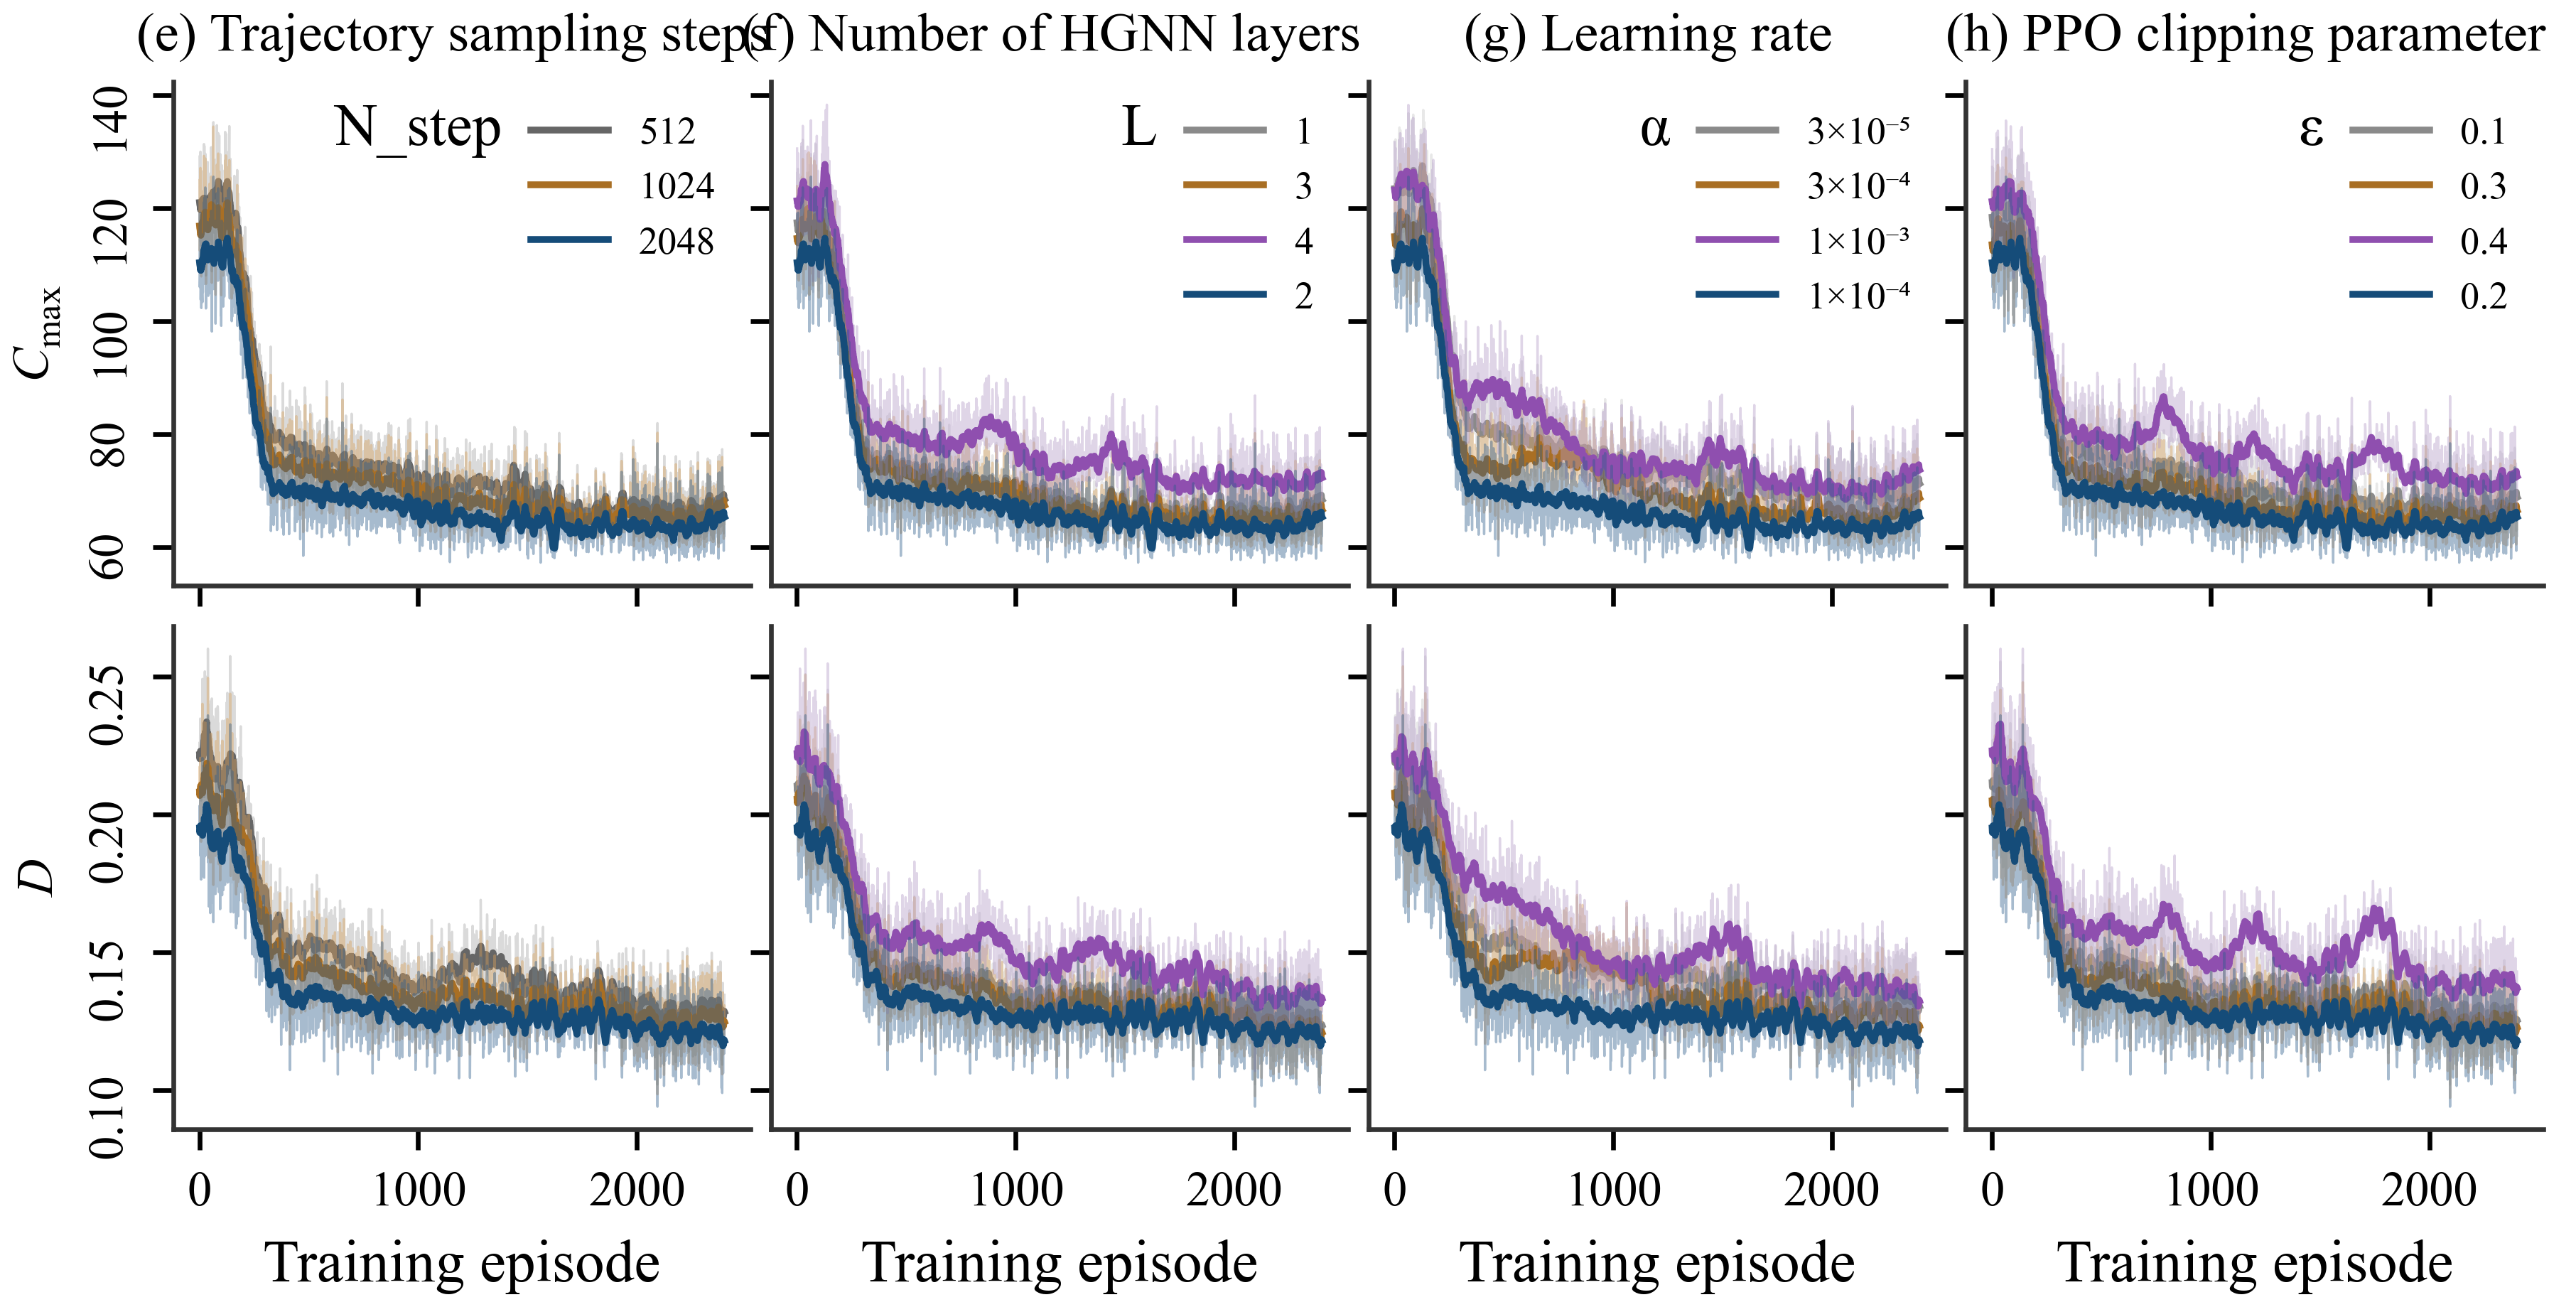
\includegraphics[width=0.85\linewidth]{figures/F5lyk敏感性参数实验图_原图.png}
    \caption{Sensitivity of HGNN-PPO to trajectory length, encoder depth, learning rate, and clipping parameter.}
    \label{fig:hyperparameter_sensitivity}
\end{figure*}

Figure~\ref{fig:hyperparameter_sensitivity} shows a rapid initial decrease in both objectives, followed
by slower improvement. Among the displayed settings, 2048 sampling steps yield lower late-training
objective curves than shorter trajectories. Two HGNN layers provide lower curves than the one-,
three-, and four-layer settings, indicating that increasing depth alone does not improve this
configuration. A learning rate of $1\times10^{-4}$ and clipping parameter of 0.2 similarly give
favorable late-training performance; the more aggressive settings show higher objective levels or
more persistent fluctuations. The subsequent configuration therefore uses 2048 steps, two HGNN layers,
a learning rate of $1\times10^{-4}$, and clipping parameter 0.2.

% 观察来自现有F5与大论文敏感性分析，不凭曲线读取精确改善百分比。
% 图支持所比较配置中的相对选择，不说明该参数组合对所有问题全局最优。
% TODO：补齐每次仅改变一个参数的控制方式、重复次数及曲线阴影定义；
% 轨迹采样步数不等同于横轴训练回合数。

\subsection{Ablation Experiment}
\label{subsec:ablation}

The ablation study focuses on the state encoder. HGNN-PPO-$\alpha$ examines the contribution of
heterogeneous graph information, while HGNN-PPO-$\beta$ examines attention within the graph-based
policy. Removing a representation component does not remove the corresponding physical constraint:
technological precedence, assembly readiness, and machine capacity remain enforced by the environment.
The instance-wise outcomes of these variants are included in
Tables~\ref{tab:ch3_strategy_effectiveness_small}--\ref{tab:ch3_strategy_effectiveness_large}.

% 只写大论文已定义的HGNN与注意力变体，不将未实施的静态图、删齐套边等
% 新消融写成已有实验。表示消融不改变环境中的物理可行性。

\begin{figure*}[!htbp]
    \centering
    \captionsetup{name=Figure}
    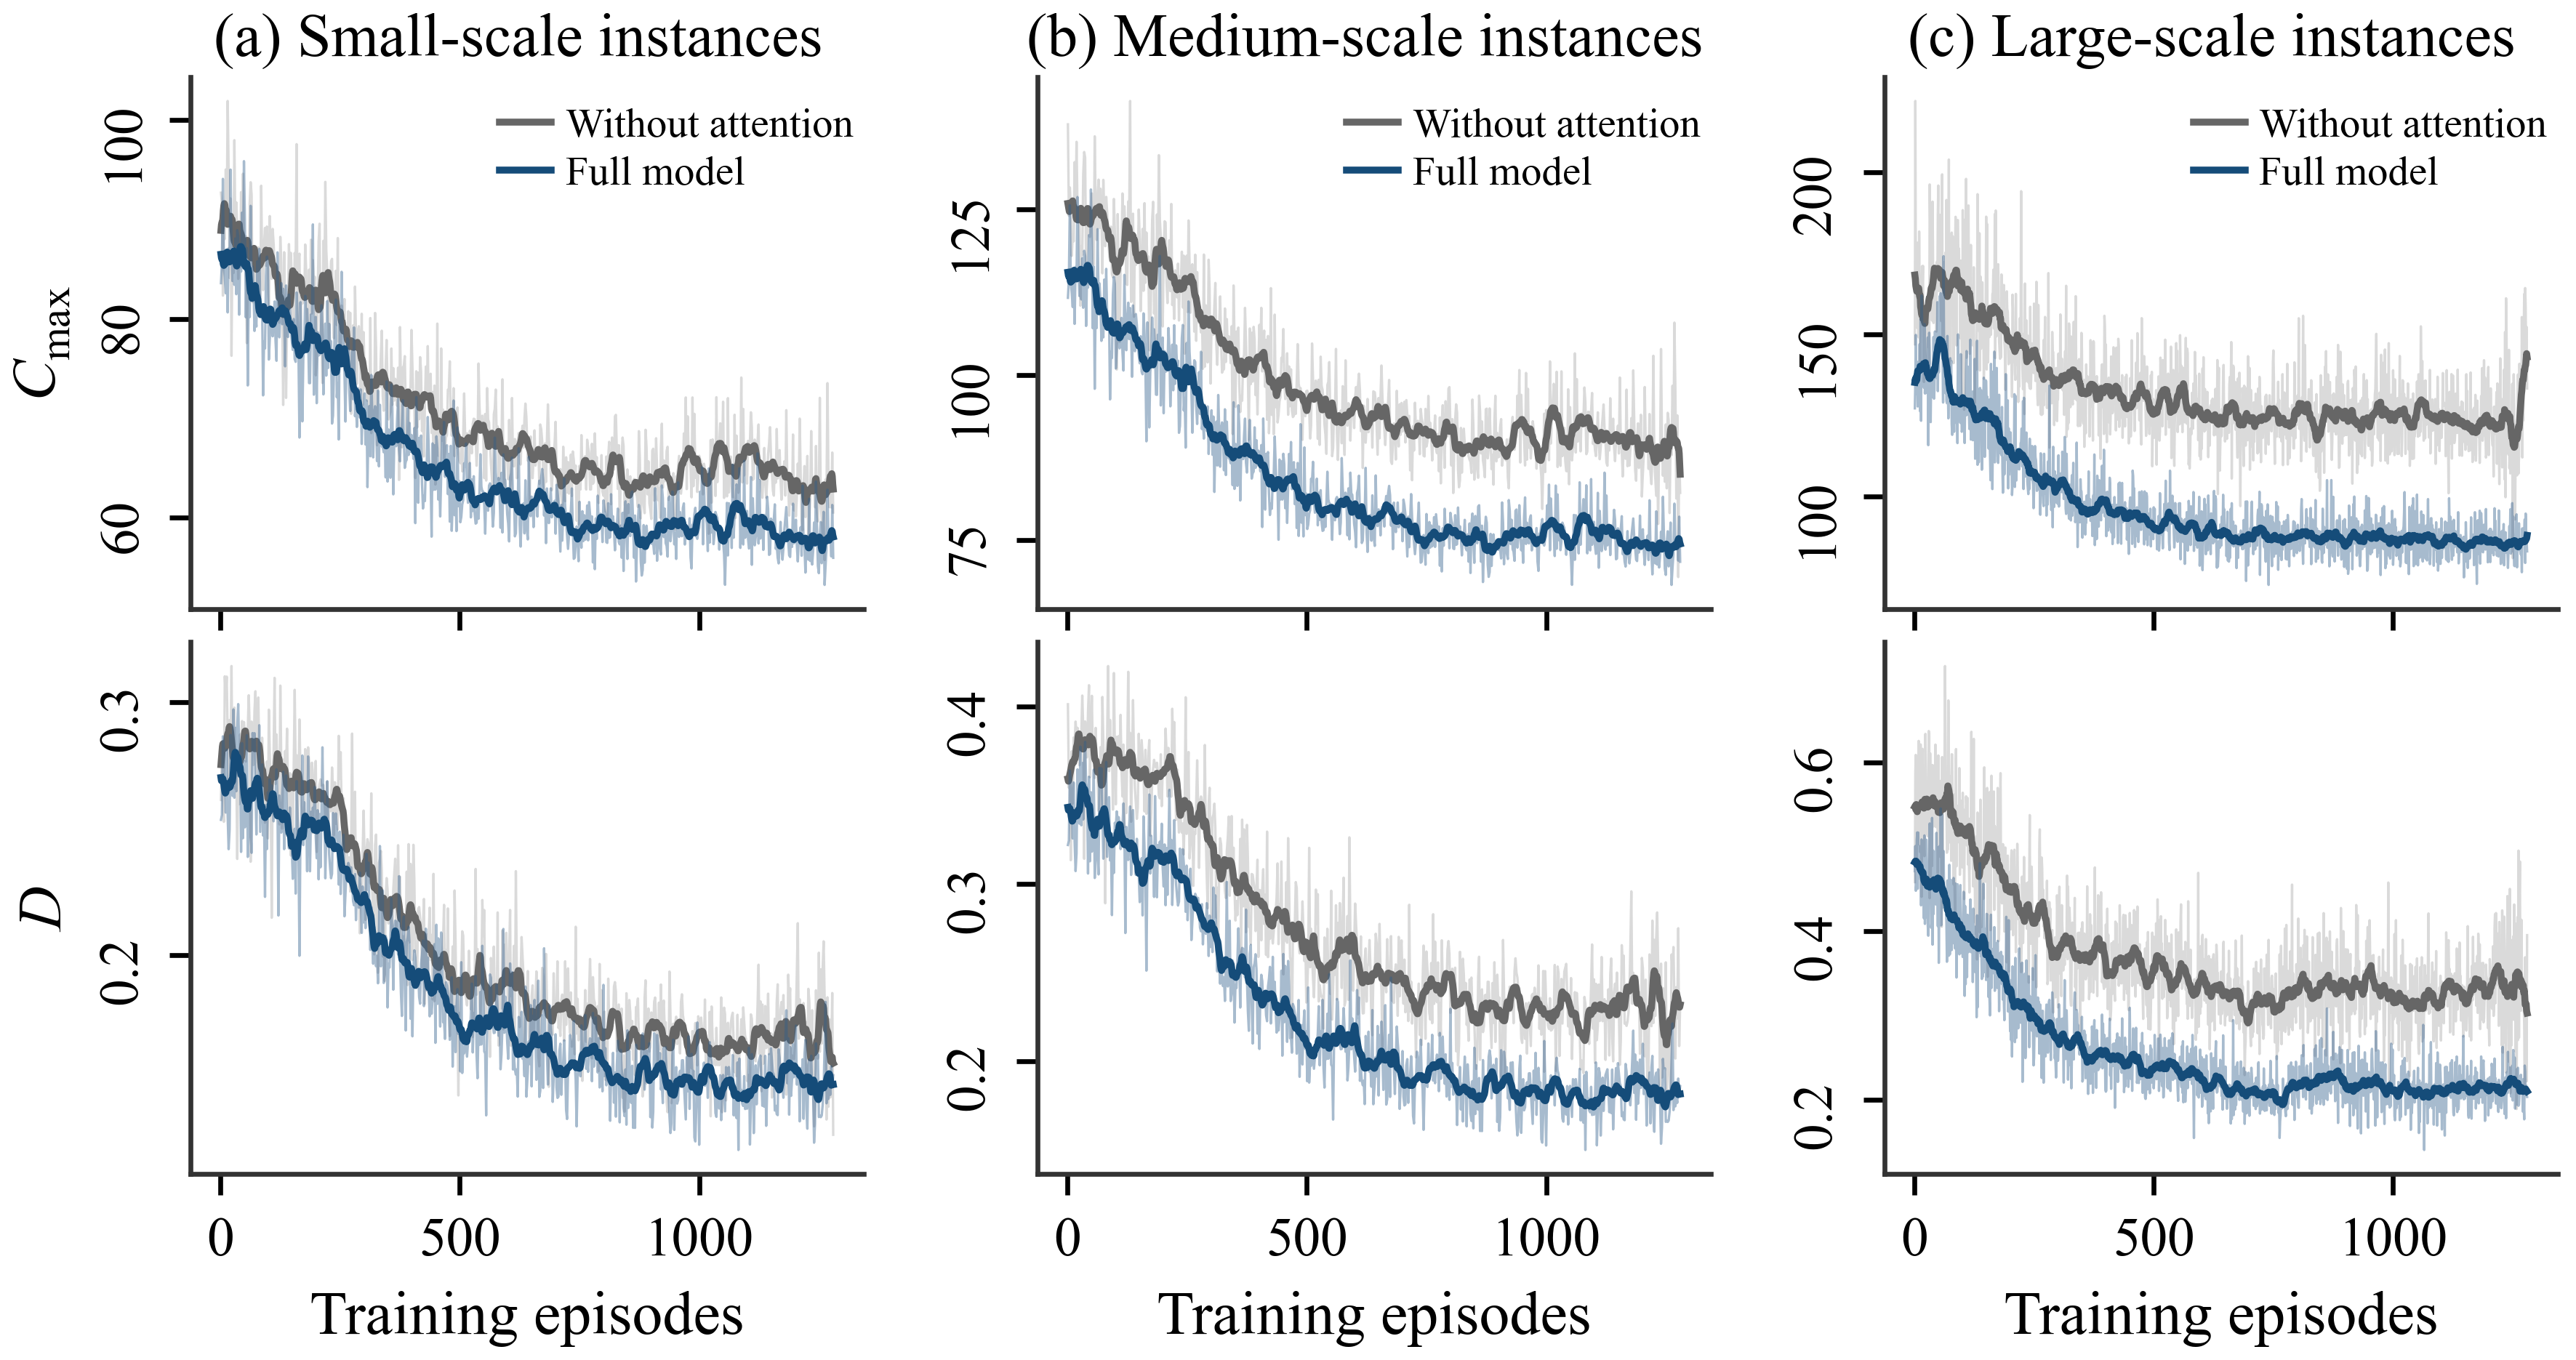
\includegraphics[width=0.85\linewidth]{figures/F7lyk大中小有无注意力机制_原图.png}
    \caption{Training performance with and without semantic attention at three instance scales.}
    \label{fig:ablation_attention_convergence}
\end{figure*}

In Fig.~\ref{fig:ablation_attention_convergence}, both configurations improve rapidly during early
training and then approach a plateau. The complete model generally reaches lower makespan and
deviation curves. The late-training separation is more pronounced in the medium and large groups
than in the small group. This pattern is consistent with a benefit from distinguishing resource and
assembly semantics when the production state contains more interacting branches. It supports the
attention configuration as a whole; it does not isolate the contribution of each individual meta-path.

% 有无注意力图中，中大规模后期差距更明显，解释为与复杂状态语义区分相符。
% 不把整体注意力消融夸大为六条元路径逐项均有效的证据。
% TODO：明确无注意力版本采用均匀融合还是其他实现，并核验共享预算和种子。

\begin{figure*}[!htbp]
    \centering
    \captionsetup{name=Figure}
    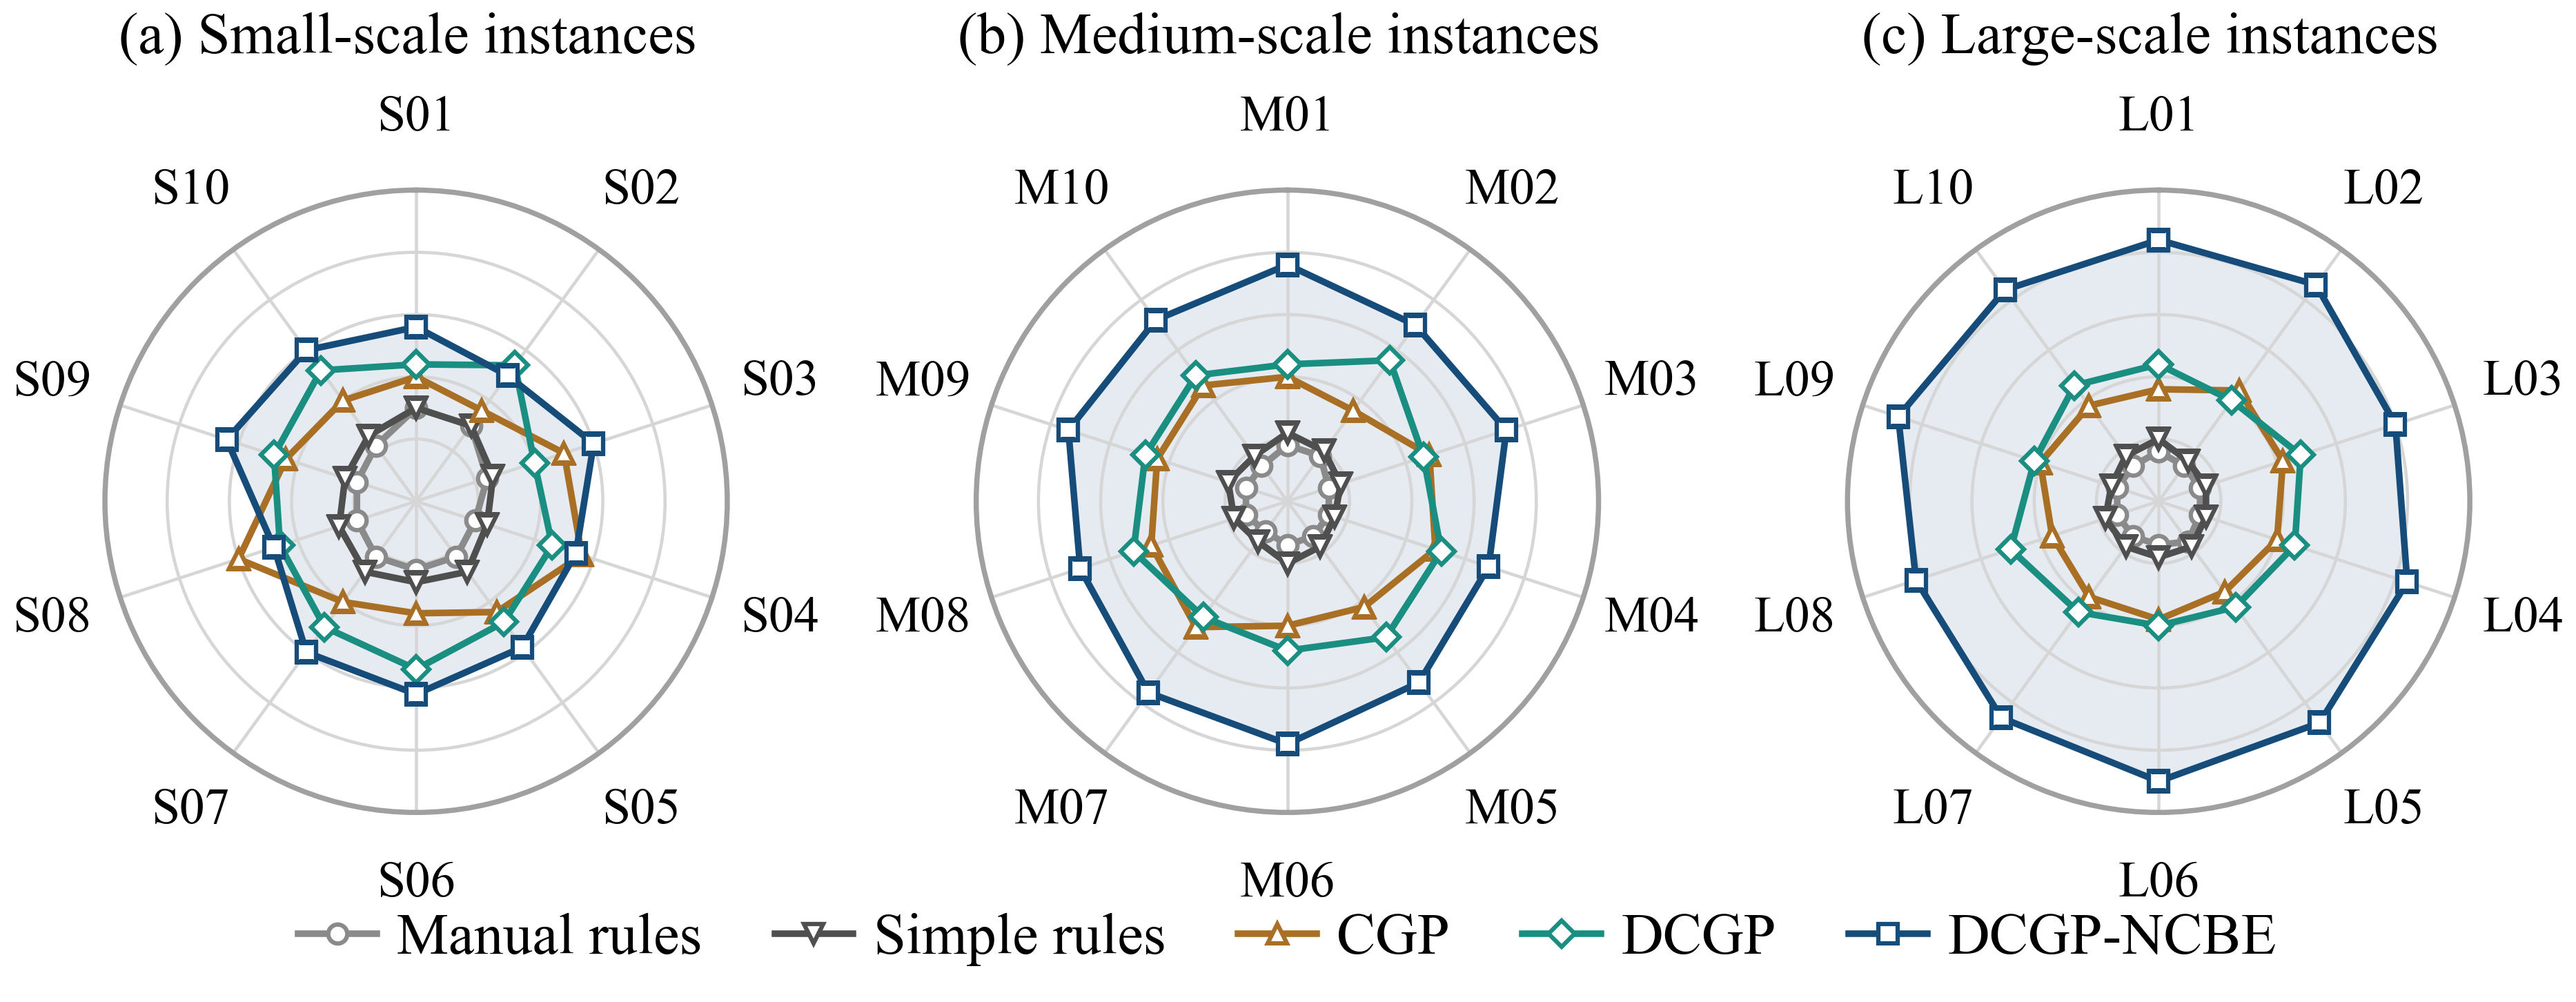
\includegraphics[width=0.85\linewidth]{figures/F8lyk不同规模算例下各类规则的选择比例_原图.png}
    \caption{Selection ratios of candidate rule families in the supplied rule-library configuration.}
    \label{fig:candidate_rule_selection}
\end{figure*}

Figure~\ref{fig:candidate_rule_selection} provides a complementary view of policy behavior under the
supplied rule pool. The displayed families comprise manual rules, simple rules, CGP, DCGP, and
DCGP-NCBE rules. Selection profiles vary across instances, while the DCGP-NCBE family occupies a
larger share in the large-scale group. The display therefore describes how the recorded selector uses
that particular candidate pool. It is not a separate ablation of the encoder, and selection frequency
alone cannot establish the causal contribution of a rule family.

% 保留原规则来源名称，不将DCGP生成方法重新包装成本文创新。
% 数据清单将此图标为未核验汇总：尚缺动作日志及各头统计分母。
% TODO：若最终使用简单基础规则库，本图必须用对应动作日志重新统计，
% 不能只替换图例或把原选择比例解释为新规则库行为。

\subsection{Result Analysis}
\label{subsec:result_analysis}
\subsubsection{Comparison on Training Instances}
\label{subsec:comparative_results}

Figure~\ref{fig:training_convergence_random_instances} reports per-episode objective values and their
20-episode moving averages. Both objectives decrease during the early training stage and improve more
slowly thereafter at all three scales. Fluctuations remain around the smoothed trend, particularly
under the larger workloads. The curves describe the learning trajectory; they are considered together
with the instance-wise comparisons and the independent tests rather than treated as independent
replications of final policy performance.

% F6图例明确给出逐回合值与20回合移动平均，因此采用这一准确描述。
% TODO：补充代表算例编号、模型偏好及各曲线是否来自同一次训练。

\begin{figure*}[!htbp]
    \centering
    \captionsetup{name=Figure}
    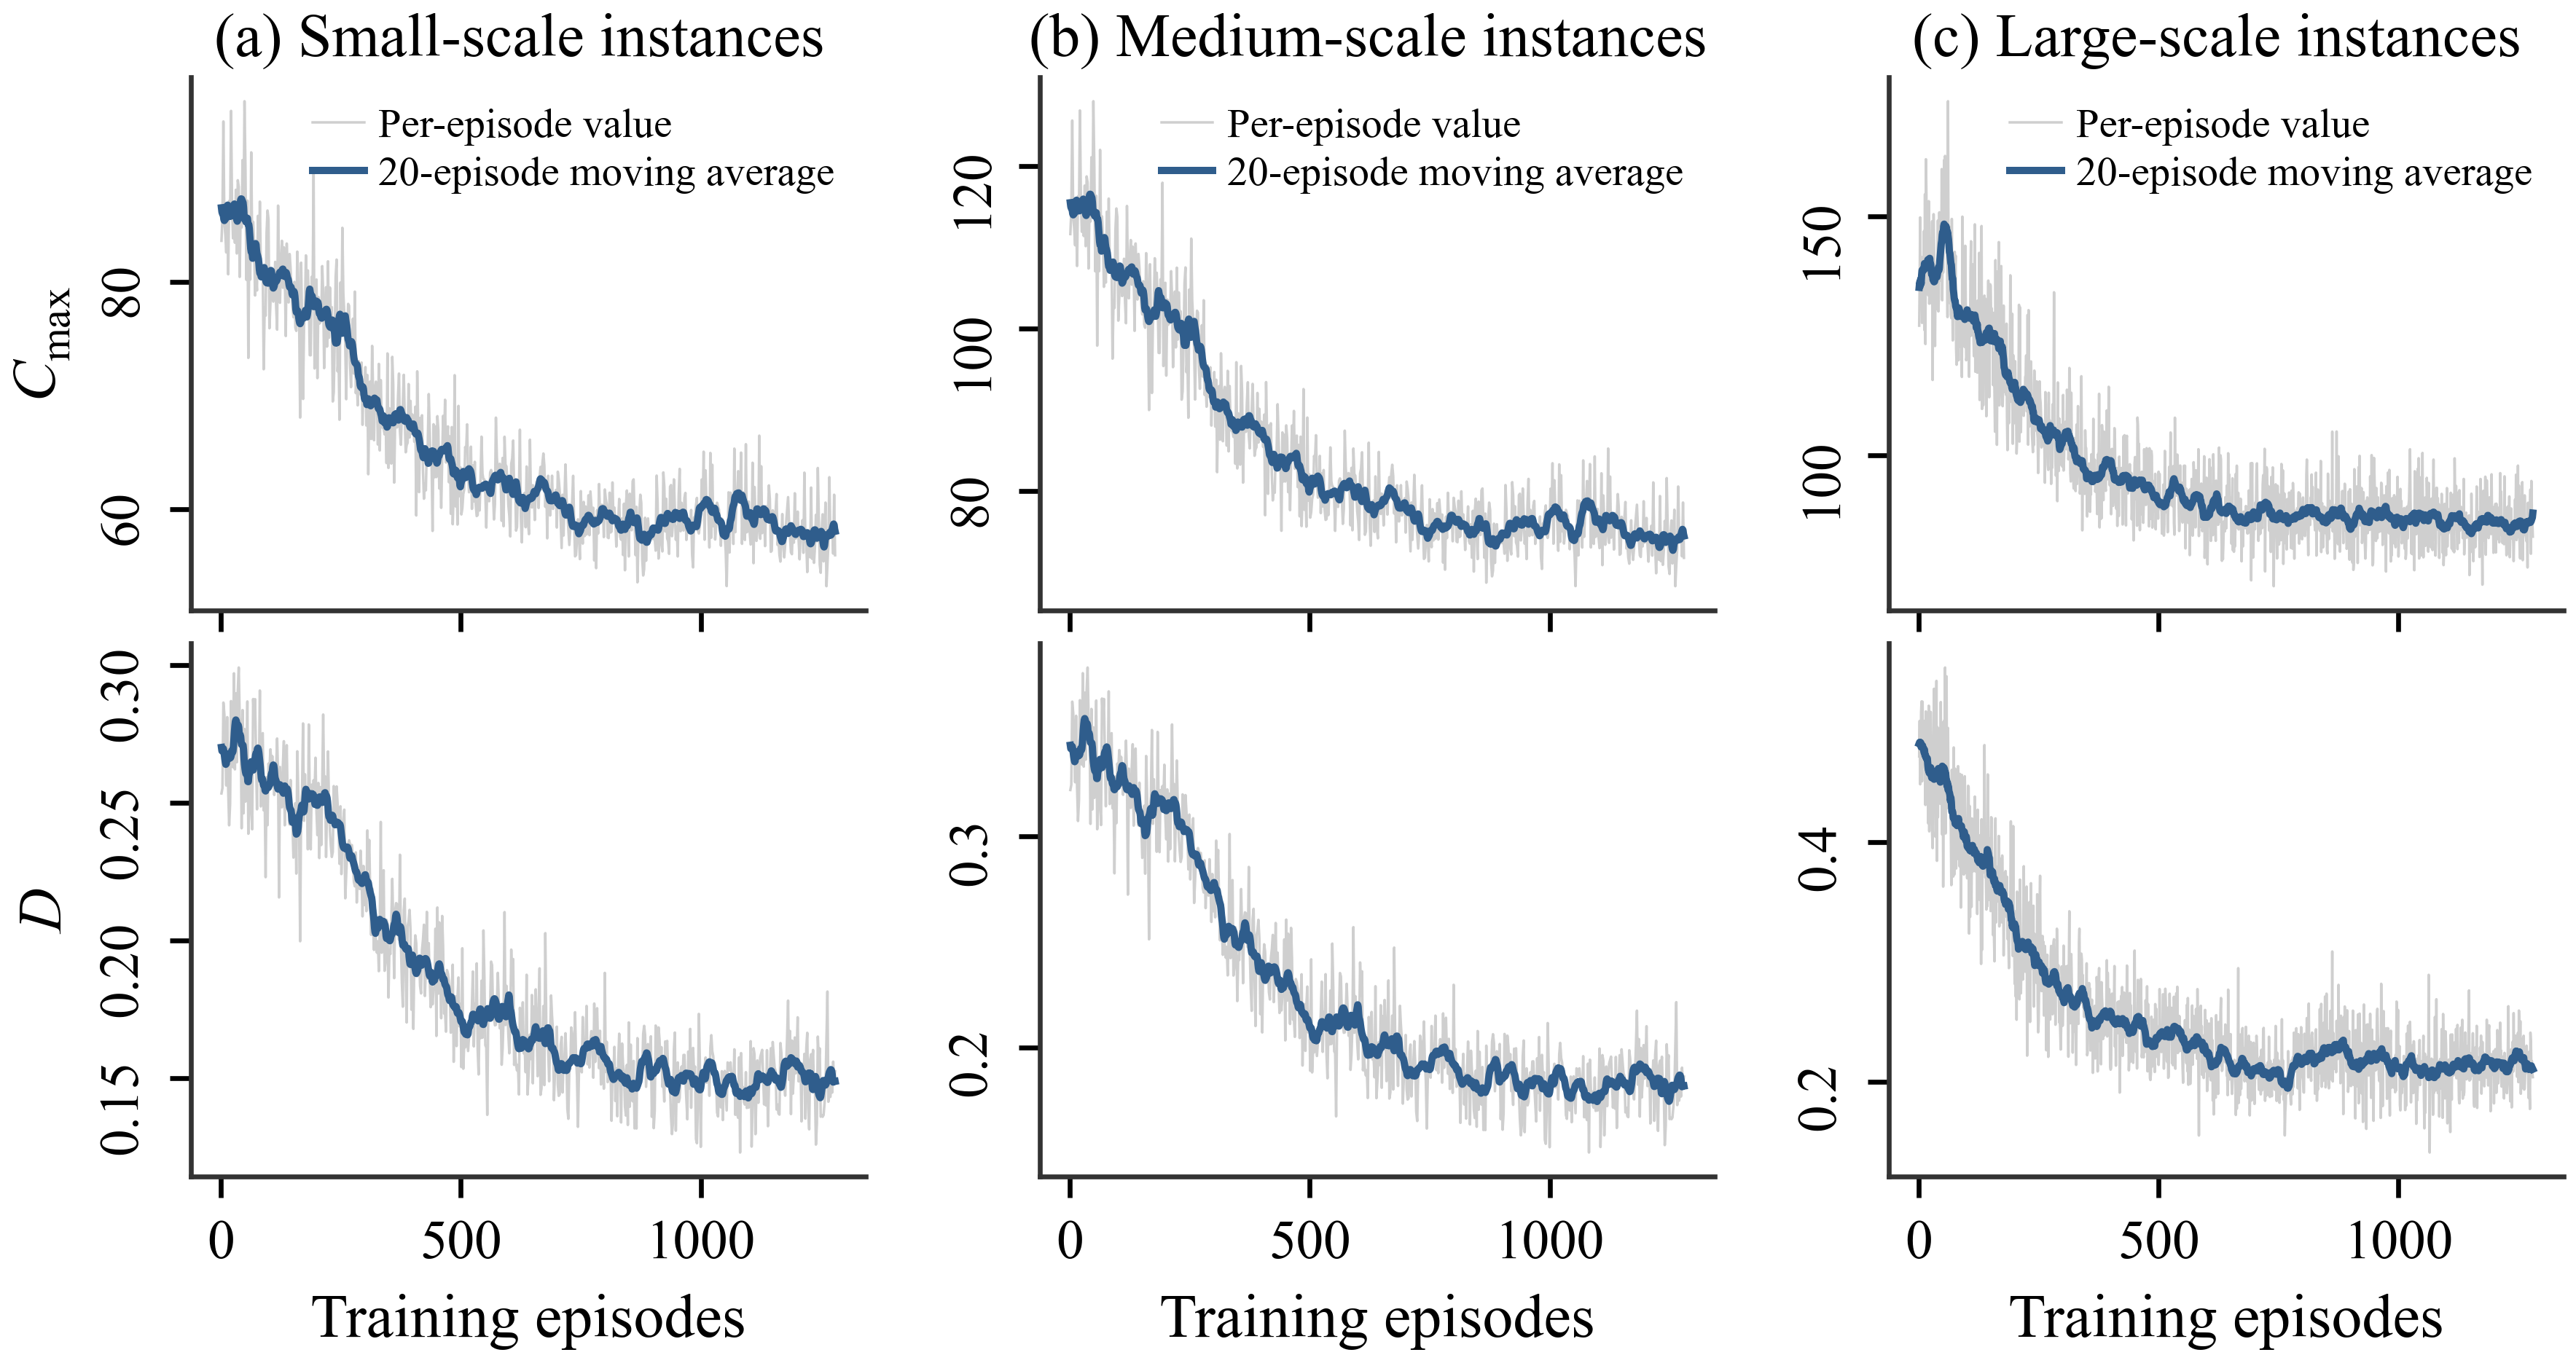
\includegraphics[width=0.85\linewidth]{figures/F6lyk强化学习训练曲线1_原图.png}
    \caption{Per-episode objectives and 20-episode moving averages during HGNN-PPO training.}
    \label{fig:training_convergence_random_instances}
\end{figure*}

\begin{table*}[!htbp]
    \centering
    \captionsetup{name=Table}
    \songti\rmfamily
% 小规模训练场景下不同策略的对比结果
    \caption{Comparison Results of Different Strategies on Small-scale Training Scenarios}
    \label{tab:ch3_strategy_effectiveness_small}
    \zihao{-5}
    \setlength{\tabcolsep}{0pt}
    \renewcommand{\arraystretch}{0.95}
    \begin{tabular*}{\textwidth}{@{\extracolsep{\fill}} c cc cc cc cc cc cc @{}}
        \toprule
        \multirow{2}{*}{Instance}
        & \multicolumn{2}{c}{HRS}
        & \multicolumn{2}{c}{ERS}
        & \multicolumn{2}{c}{DQN}
        & \multicolumn{2}{c}{HGNN-PPO-$\alpha$}
        & \multicolumn{2}{c}{HGNN-PPO-$\beta$}
        & \multicolumn{2}{c}{HGNN-PPO}
        \\
        \cmidrule(lr){2-3}
        \cmidrule(lr){4-5}
        \cmidrule(lr){6-7}
        \cmidrule(lr){8-9}
        \cmidrule(lr){10-11}
        \cmidrule(lr){12-13}
        & $C_{\max}$ & $D_{\mathrm{dev}}$
        & $C_{\max}$ & $D_{\mathrm{dev}}$
        & $C_{\max}$ & $D_{\mathrm{dev}}$
        & $C_{\max}$ & $D_{\mathrm{dev}}$
        & $C_{\max}$ & $D_{\mathrm{dev}}$
        & $C_{\max}$ & $D_{\mathrm{dev}}$
        \\
        \midrule
        TR\_S01 & 99.40 & \underline{53.89} & 95.19 & 69.66 & 93.75 & 76.23 & 92.32 & 63.09 & \underline{90.89} & \textbf{49.95} & \textbf{89.46} & 57.83 \\
        TR\_S02 & 48.70 & 111.87 & \underline{41.76} & 100.51 & \textbf{40.69} & 80.06 & 43.90 & 89.15 & 44.97 & \underline{73.24} & 42.83 & \textbf{66.42} \\
        TR\_S03 & 57.38 & 121.34 & 54.94 & 80.39 & 54.12 & 106.72 & 53.29 & 92.09 & \underline{52.47} & \underline{71.62} & \textbf{51.64} & \textbf{62.84} \\
        TR\_S04 & 60.11 & 167.16 & 52.78 & 118.99 & 50.33 & 143.08 & \textbf{47.87} & \textbf{70.82} & 51.56 & \underline{85.27} & \underline{49.10} & 99.72 \\
        TR\_S05 & 76.80 & 135.92 & 73.54 & 90.29 & 72.44 & 72.03 & 71.33 & \textbf{44.65} & \underline{70.23} & 113.10 & \textbf{69.12} & \underline{58.34} \\
        TR\_S06 & 58.32 & 119.79 & 51.75 & 106.10 & 49.23 & \textbf{78.72} & \textbf{46.70} & 133.48 & \underline{47.97} & 95.15 & 50.49 & \underline{86.93} \\
        TR\_S07 & 92.15 & 91.85 & 88.67 & 81.51 & 87.49 & 62.89 & 86.31 & \underline{56.69} & \underline{85.12} & \textbf{50.48} & \textbf{83.94} & 71.17 \\
        TR\_S08 & 57.49 & 120.63 & 54.33 & 106.86 & 53.03 & \textbf{65.56} & \underline{50.45} & 82.08 & \textbf{49.15} & 93.10 & 51.74 & \underline{73.82} \\
        TR\_S09 & 70.16 & 126.88 & 66.93 & 145.17 & 64.40 & \underline{82.98} & \textbf{61.88} & 108.59 & 65.67 & 93.95 & \underline{63.14} & \textbf{72.00} \\
        TR\_S10 & 53.19 & 121.65 & 50.93 & 104.57 & 50.17 & 138.74 & 49.40 & 90.90 & \underline{48.64} & \underline{80.64} & \textbf{47.87} & \textbf{70.39} \\
        \midrule
        Best count & 0/10 & 0/10 & 0/10 & 0/10 & 1/10 & 2/10 & 3/10 & 2/10 & 1/10 & 2/10 & 5/10 & 4/10 \\
        Top-two count & 0/10 & 1/10 & 1/10 & 0/10 & 1/10 & 3/10 & 4/10 & 3/10 & 7/10 & 6/10 & 7/10 & 7/10 \\
        Overall rank & \multicolumn{2}{c}{6} & \multicolumn{2}{c}{5} & \multicolumn{2}{c}{4} & \multicolumn{2}{c}{3} & \multicolumn{2}{c}{2} & \multicolumn{2}{c}{1} \\
        \bottomrule
    \end{tabular*}
\end{table*}

For the small-scale group in Table~\ref{tab:ch3_strategy_effectiveness_small}, HGNN-PPO obtains the
lowest makespan on five instances and the lowest deviation on four, with seven top-two placements
for each objective. On TR\_S03, for example, its $(C_{\max},D_{\mathrm{dev}})$ values are
$(51.64,62.84)$, compared with $(52.47,71.62)$ for the no-attention variant. The advantage is not
uniform: DQN gives the shortest makespan on TR\_S02, and HGNN-PPO-$\alpha$ gives the best values
for both objectives on TR\_S04. The results therefore favor adaptive state encoding in aggregate
without implying dominance on every small instance.

% 本段数值直接来自当前小论文表，未照搬大论文中略有不同的工期数值。

\begin{table*}[!htbp]
    \centering
    \captionsetup{name=Table}
    \songti\rmfamily
% 中规模训练场景下不同策略的对比结果
    \caption{Comparison Results of Different Strategies on Medium-scale Training Scenarios}
    \label{tab:ch3_strategy_effectiveness_medium}
    \zihao{-5}
    \setlength{\tabcolsep}{0pt}
    \renewcommand{\arraystretch}{0.95}
    \begin{tabular*}{\textwidth}{@{\extracolsep{\fill}} c cc cc cc cc cc cc @{}}
        \toprule
        \multirow{2}{*}{Instance}
        & \multicolumn{2}{c}{HRS}
        & \multicolumn{2}{c}{ERS}
        & \multicolumn{2}{c}{DQN}
        & \multicolumn{2}{c}{HGNN-PPO-$\alpha$}
        & \multicolumn{2}{c}{HGNN-PPO-$\beta$}
        & \multicolumn{2}{c}{HGNN-PPO}
        \\
        \cmidrule(lr){2-3}
        \cmidrule(lr){4-5}
        \cmidrule(lr){6-7}
        \cmidrule(lr){8-9}
        \cmidrule(lr){10-11}
        \cmidrule(lr){12-13}
        & $C_{\max}$ & $D_{\mathrm{dev}}$
        & $C_{\max}$ & $D_{\mathrm{dev}}$
        & $C_{\max}$ & $D_{\mathrm{dev}}$
        & $C_{\max}$ & $D_{\mathrm{dev}}$
        & $C_{\max}$ & $D_{\mathrm{dev}}$
        & $C_{\max}$ & $D_{\mathrm{dev}}$
        \\
        \midrule
        TR\_M01 & \underline{59.07} & 123.29 & 61.86 & 148.19 & 60.93 & 78.48 & 60.00 & \underline{63.54} & 64.60 & \textbf{48.60} & \textbf{58.14} & 98.40 \\
        TR\_M02 & 61.72 & 186.82 & 58.88 & 153.03 & \textbf{54.43} & 119.24 & 57.77 & \textbf{51.66} & 56.65 & \underline{71.93} & \underline{55.54} & 92.21 \\
        TR\_M03 & 68.00 & 181.16 & 65.12 & \underline{78.18} & 64.14 & \textbf{62.61} & 63.16 & 151.52 & \underline{62.18} & 80.39 & \textbf{61.20} & 94.89 \\
        TR\_M04 & 58.70 & 170.12 & 52.02 & 173.53 & 50.84 & 128.71 & 49.65 & \textbf{45.89} & \underline{48.47} & 95.58 & \textbf{47.29} & \underline{70.74} \\
        TR\_M05 & 64.90 & 177.08 & \textbf{53.30} & 138.10 & \underline{54.71} & 67.94 & 57.51 & 99.12 & 58.92 & \textbf{21.16} & 56.11 & \underline{44.55} \\
        TR\_M06 & 67.22 & 180.15 & 63.80 & 104.71 & 62.64 & 74.53 & 61.47 & 142.43 & \underline{60.31} & \underline{51.90} & \textbf{59.15} & \textbf{29.27} \\
        TR\_M07 & 72.72 & 88.41 & 69.02 & 136.39 & 67.76 & 109.73 & 66.50 & \underline{72.41} & \underline{65.25} & 163.04 & \textbf{63.99} & \textbf{56.42} \\
        TR\_M08 & 64.60 & 166.76 & 61.04 & 113.82 & 59.64 & 196.17 & 58.25 & 137.35 & \textbf{55.46} & \underline{96.17} & \underline{56.85} & \textbf{78.52} \\
        TR\_M09 & 59.71 & 205.13 & 56.67 & 107.39 & 55.64 & \textbf{65.50} & 54.61 & 135.32 & \underline{53.58} & 170.22 & \textbf{52.55} & \underline{86.44} \\
        TR\_M10 & 58.32 & \textbf{64.14} & 55.35 & 125.16 & 54.34 & 186.18 & 53.34 & \underline{82.45} & \underline{52.33} & 155.67 & \textbf{51.32} & 90.75 \\
        \midrule
        Best count & 0/10 & 1/10 & 1/10 & 0/10 & 1/10 & 2/10 & 0/10 & 2/10 & 1/10 & 2/10 & 7/10 & 3/10 \\
        Top-two count & 1/10 & 1/10 & 1/10 & 1/10 & 2/10 & 2/10 & 0/10 & 5/10 & 7/10 & 5/10 & 9/10 & 6/10 \\
        Overall rank & \multicolumn{2}{c}{6} & \multicolumn{2}{c}{5} & \multicolumn{2}{c}{4} & \multicolumn{2}{c}{3} & \multicolumn{2}{c}{2} & \multicolumn{2}{c}{1} \\
        \bottomrule
    \end{tabular*}
\end{table*}

The medium-scale results in Table~\ref{tab:ch3_strategy_effectiveness_medium} show seven best
makespan values and nine top-two placements for HGNN-PPO. Its deviation is best on three instances
and among the top two on six. On TR\_M06, the complete model gives $(59.15,29.27)$, improving
both displayed objectives relative to the no-attention values $(60.31,51.90)$. By contrast, on
TR\_M01, the complete model gives the shortest makespan but a higher deviation than either
HGNN-PPO variant. This contrast highlights the need to inspect both objectives rather than infer
plan stability from completion time alone.

% 中规模突出完工效率，并用M01说明两目标并非处处同步改善。

\begin{table*}[!htbp]
    \centering
    \captionsetup{name=Table}
    \songti\rmfamily
% 大规模训练场景下不同策略的对比结果
    \caption{Comparison Results of Different Strategies on Large-scale Training Scenarios}
    \label{tab:ch3_strategy_effectiveness_large}
    \zihao{-5}
    \setlength{\tabcolsep}{0pt}
    \renewcommand{\arraystretch}{0.95}
    \begin{tabular*}{\textwidth}{@{\extracolsep{\fill}} c cc cc cc cc cc cc @{}}
        \toprule
        \multirow{2}{*}{Instance}
        & \multicolumn{2}{c}{HRS}
        & \multicolumn{2}{c}{ERS}
        & \multicolumn{2}{c}{DQN}
        & \multicolumn{2}{c}{HGNN-PPO-$\alpha$}
        & \multicolumn{2}{c}{HGNN-PPO-$\beta$}
        & \multicolumn{2}{c}{HGNN-PPO}
        \\
        \cmidrule(lr){2-3}
        \cmidrule(lr){4-5}
        \cmidrule(lr){6-7}
        \cmidrule(lr){8-9}
        \cmidrule(lr){10-11}
        \cmidrule(lr){12-13}
        & $C_{\max}$ & $D_{\mathrm{dev}}$
        & $C_{\max}$ & $D_{\mathrm{dev}}$
        & $C_{\max}$ & $D_{\mathrm{dev}}$
        & $C_{\max}$ & $D_{\mathrm{dev}}$
        & $C_{\max}$ & $D_{\mathrm{dev}}$
        & $C_{\max}$ & $D_{\mathrm{dev}}$
        \\
        \midrule
        TR\_L01 & 89.70 & 176.84 & 84.75 & 216.54 & 82.81 & 105.39 & 80.88 & 137.15 & \textbf{77.00} & \textbf{57.75} & \underline{78.94} & \underline{81.57} \\
        TR\_L02 & 91.01 & \underline{67.95} & 78.60 & 121.21 & 76.81 & 197.29 & 75.02 & 90.77 & \underline{73.24} & 159.25 & \textbf{71.45} & \textbf{45.12} \\
        TR\_L03 & 88.10 & 185.26 & 75.59 & \underline{74.44} & 73.87 & 152.67 & 72.16 & 93.99 & \underline{70.44} & 80.07 & \textbf{68.72} & \textbf{54.88} \\
        TR\_L04 & 93.42 & 124.44 & 75.98 & \textbf{53.57} & \underline{70.55} & 134.15 & 74.17 & 101.92 & \textbf{68.74} & 179.73 & 72.36 & \underline{77.74} \\
        TR\_L05 & 89.30 & 179.28 & 85.12 & 149.46 & 83.70 & \underline{77.88} & 82.28 & 95.78 & \underline{80.86} & \textbf{59.99} & \textbf{79.44} & 87.64 \\
        TR\_L06 & 58.40 & 161.94 & 56.25 & 133.71 & 55.40 & 105.48 & \textbf{52.88} & \textbf{49.02} & 54.56 & 82.90 & \underline{53.72} & \underline{65.96} \\
        TR\_L07 & 92.00 & 109.66 & 80.96 & 205.17 & 79.12 & 171.06 & 77.28 & 136.95 & \underline{75.44} & \textbf{68.73} & \textbf{73.60} & \underline{89.20} \\
        TR\_L08 & 94.27 & 151.18 & 82.96 & \underline{94.36} & 81.08 & 218.06 & 79.19 & \textbf{84.29} & \underline{77.31} & 184.62 & \textbf{75.42} & 98.42 \\
        TR\_L09 & 109.37 & 125.51 & 99.44 & 209.43 & 94.81 & 91.94 & \textbf{90.19} & 167.47 & 97.13 & \textbf{41.59} & \underline{92.50} & \underline{66.77} \\
        TR\_L10 & 96.52 & 153.38 & 87.14 & 126.73 & 85.16 & \textbf{46.78} & 83.18 & 100.08 & \underline{81.20} & \underline{62.77} & \textbf{79.22} & 78.76 \\
        \midrule
        Best count & 0/10 & 0/10 & 0/10 & 1/10 & 0/10 & 1/10 & 2/10 & 2/10 & 2/10 & 4/10 & 6/10 & 2/10 \\
        Top-two count & 0/10 & 1/10 & 0/10 & 3/10 & 1/10 & 2/10 & 2/10 & 2/10 & 8/10 & 5/10 & 9/10 & 7/10 \\
        Overall rank & \multicolumn{2}{c}{6} & \multicolumn{2}{c}{5} & \multicolumn{2}{c}{4} & \multicolumn{2}{c}{3} & \multicolumn{2}{c}{2} & \multicolumn{2}{c}{1} \\
        \bottomrule
    \end{tabular*}
\end{table*}

For large instances in Table~\ref{tab:ch3_strategy_effectiveness_large}, HGNN-PPO obtains six best
makespan values and nine top-two placements. Its deviation is best on two instances but among the
top two on seven. On TR\_L02, it achieves $(71.45,45.12)$, whereas the no-attention variant gives
$(73.24,159.25)$. On TR\_L01, however, the no-attention variant is better on both objectives.
Across the 30 displayed instances, the complete model records 18 best makespan values and nine
best deviation values. Thus its most consistent instance-wise advantage concerns makespan, while
the stability benefit depends more strongly on the scenario.

% 最优次数按三张表逐行核算：工期18/30，偏离度9/30。
% 综合排名原样保留，但排名公式尚缺，因此不以第一名替代目标值分析。
% TODO：补齐代表值筛选规则、均值或中位数定义、独立运行及不确定性。

\subsubsection{Generalization Experiment on Independent Test Instances}
\label{subsec:generalization_runtime}

The independent evaluation applies frozen policies to 15 test instances, five at each scale. Unlike
the training-instance analysis, it examines solution sets obtained on instances outside the learning
partition. Table~\ref{tab:ch3_rl_generalization_result} summarizes HV and Spread, while
Figs.~\ref{fig:pareto_front_unseen_scenarios} and~\ref{fig:objective_distributions_test_scenarios}
show representative trade-offs and objective distributions. These plots serve different purposes:
the front display identifies nondominated alternatives, whereas the distribution display shows
where sampled objective values are concentrated.

% 未见算例不自动等同跨规模、跨拓扑或跨分布，正文不作这些未经证实的外推。
% TODO：补齐训练模型到测试算例的对应关系与测试重复次数。

\begin{table*}[!htbp]
    \centering
    \captionsetup{name=Table}
    \songti\rmfamily
% 不同算法在独立测试算例上的HV和Spread
    \caption{HV and Spread of Different Algorithms on Independent Test Instances}
    \label{tab:ch3_rl_generalization_result}
    \zihao{-5}
    \setlength{\tabcolsep}{0pt}
    \renewcommand{\arraystretch}{0.95}
    \begin{tabular*}{\textwidth}{
        @{\extracolsep{\fill}} c
        cc cc cc cc cc cc
        @{}
    }
        \toprule
        \multirow{2}{*}{Instance}
        & \multicolumn{2}{c}{L2D}
        & \multicolumn{2}{c}{\makecell[c]{MPGN-\\MPPO}}
        & \multicolumn{2}{c}{\makecell[c]{GNN-\\DRL}}
        & \multicolumn{2}{c}{\makecell[c]{HGNNR-\\DRL}}
        & \multicolumn{2}{c}{\makecell[c]{MHGNN-\\SAC}}
        & \multicolumn{2}{c}{HGNN-PPO} \\
        \cmidrule(lr){2-3}
        \cmidrule(lr){4-5}
        \cmidrule(lr){6-7}
        \cmidrule(lr){8-9}
        \cmidrule(lr){10-11}
        \cmidrule(lr){12-13}
        & HV & Spread
        & HV & Spread
        & HV & Spread
        & HV & Spread
        & HV & Spread
        & HV & Spread \\
        \midrule
        \multicolumn{13}{@{}l}{Small-scale instances} \\
        S\_01 & 0.528 & 0.893 & 0.742 & 0.928 & 0.701 & 0.686 & 0.892 & \underline{0.658} & \textbf{1.130} & \textbf{0.529} & \underline{1.014} & 0.823 \\
        S\_02 & \underline{1.117} & \underline{0.478} & 0.487 & 0.971 & 0.770 & 0.930 & 1.008 & 0.789 & 0.835 & 0.876 & \textbf{1.194} & \textbf{0.361} \\
        S\_03 & 0.740 & 0.711 & 0.826 & 0.864 & 0.898 & \underline{0.557} & 0.953 & 0.636 & \textbf{1.134} & \textbf{0.549} & \underline{1.013} & 0.566 \\
        S\_04 & 0.663 & 0.850 & 0.797 & 0.917 & 1.055 & \textbf{0.518} & 1.015 & 0.735 & \underline{1.072} & \underline{0.669} & \textbf{1.206} & 0.688 \\
        S\_05 & 0.843 & \underline{0.750} & 0.524 & 0.942 & 0.930 & 0.815 & \textbf{1.142} & \textbf{0.411} & 0.922 & 0.807 & \underline{0.936} & 0.781 \\
        \midrule
        \multicolumn{13}{@{}l}{Medium-scale instances} \\
        M\_01 & 0.674 & 0.733 & 0.888 & 0.859 & 0.896 & \textbf{0.636} & 1.103 & \underline{0.724} & \underline{1.143} & 0.734 & \textbf{1.180} & 0.889 \\
        M\_02 & 0.918 & 0.768 & 0.992 & 0.809 & \underline{1.137} & 0.961 & 1.106 & \textbf{0.591} & \textbf{1.192} & \underline{0.660} & 1.135 & 0.702 \\
        M\_03 & 0.697 & 0.863 & 0.880 & 0.773 & 0.932 & 0.802 & \underline{1.107} & 0.808 & 1.070 & \underline{0.625} & \textbf{1.206} & \textbf{0.000} \\
        M\_04 & 1.064 & 0.716 & 0.863 & 0.729 & 1.105 & \textbf{0.425} & \underline{1.105} & 0.866 & 1.075 & \underline{0.622} & \textbf{1.131} & 0.728 \\
        M\_05 & 0.849 & 0.884 & 0.808 & 0.810 & 0.916 & 0.903 & 0.982 & \textbf{0.702} & \underline{1.000} & 1.026 & \textbf{1.144} & \underline{0.728} \\
        \midrule
        \multicolumn{13}{@{}l}{Large-scale instances} \\
        L\_01 & 0.598 & 0.902 & 0.834 & 0.828 & 1.114 & 0.801 & \textbf{1.208} & 0.803 & \underline{1.153} & \underline{0.713} & 1.134 & \textbf{0.668} \\
        L\_02 & 0.577 & 0.867 & 0.836 & \underline{0.501} & \textbf{1.084} & 0.787 & 0.906 & \textbf{0.440} & 1.026 & 0.932 & \underline{1.060} & 0.927 \\
        L\_03 & 0.735 & 0.766 & 0.925 & \textbf{0.721} & 0.825 & 0.812 & 1.007 & 0.889 & \textbf{1.157} & 0.800 & \underline{1.093} & \underline{0.760} \\
        L\_04 & 0.600 & 0.773 & 0.806 & 0.879 & 1.019 & \underline{0.639} & 1.028 & 1.030 & \underline{1.091} & \textbf{0.363} & \textbf{1.142} & 0.964 \\
        L\_05 & 0.919 & 0.822 & 0.685 & 0.817 & 1.080 & 0.799 & 0.980 & 0.841 & \underline{1.080} & \underline{0.764} & \textbf{1.195} & \textbf{0.679} \\
        \midrule
        Mean & 0.768 & 0.785 & 0.793 & 0.823 & 0.964 & 0.738 & 1.036 & 0.728 & \underline{1.072} & \underline{0.711} & \textbf{1.119} & \textbf{0.684} \\
        Overall rank & \multicolumn{2}{c}{5} & \multicolumn{2}{c}{6} & \multicolumn{2}{c}{4} & \multicolumn{2}{c}{3} & \multicolumn{2}{c}{2} & \multicolumn{2}{c}{1} \\
        \bottomrule
    \end{tabular*}
\end{table*}

HGNN-PPO has the highest reported average HV, 1.119, and the lowest average Spread, 0.684.
Relative to MHGNN-SAC, whose averages are 1.072 and 0.711, these correspond to approximately
4.4\% higher HV and 3.8\% lower Spread. The complete method attains the highest HV on eight of
the 15 instances, including four of the five medium-scale cases. The result is not uniform across
metrics: it attains the lowest Spread on four cases, with other methods giving more uniform sets
on several instances. Coverage and distribution should therefore be interpreted separately.

% 均值、8次最优HV与4次最优Spread均按当前15行表格核算。
% TODO：M03的Spread=0.000需结合公式、点数与退化解集规则解释，不能
% 直接称为完美分布；表内原数值保留。

\begin{figure*}[!htbp]
    \centering
    \captionsetup{name=Figure}
    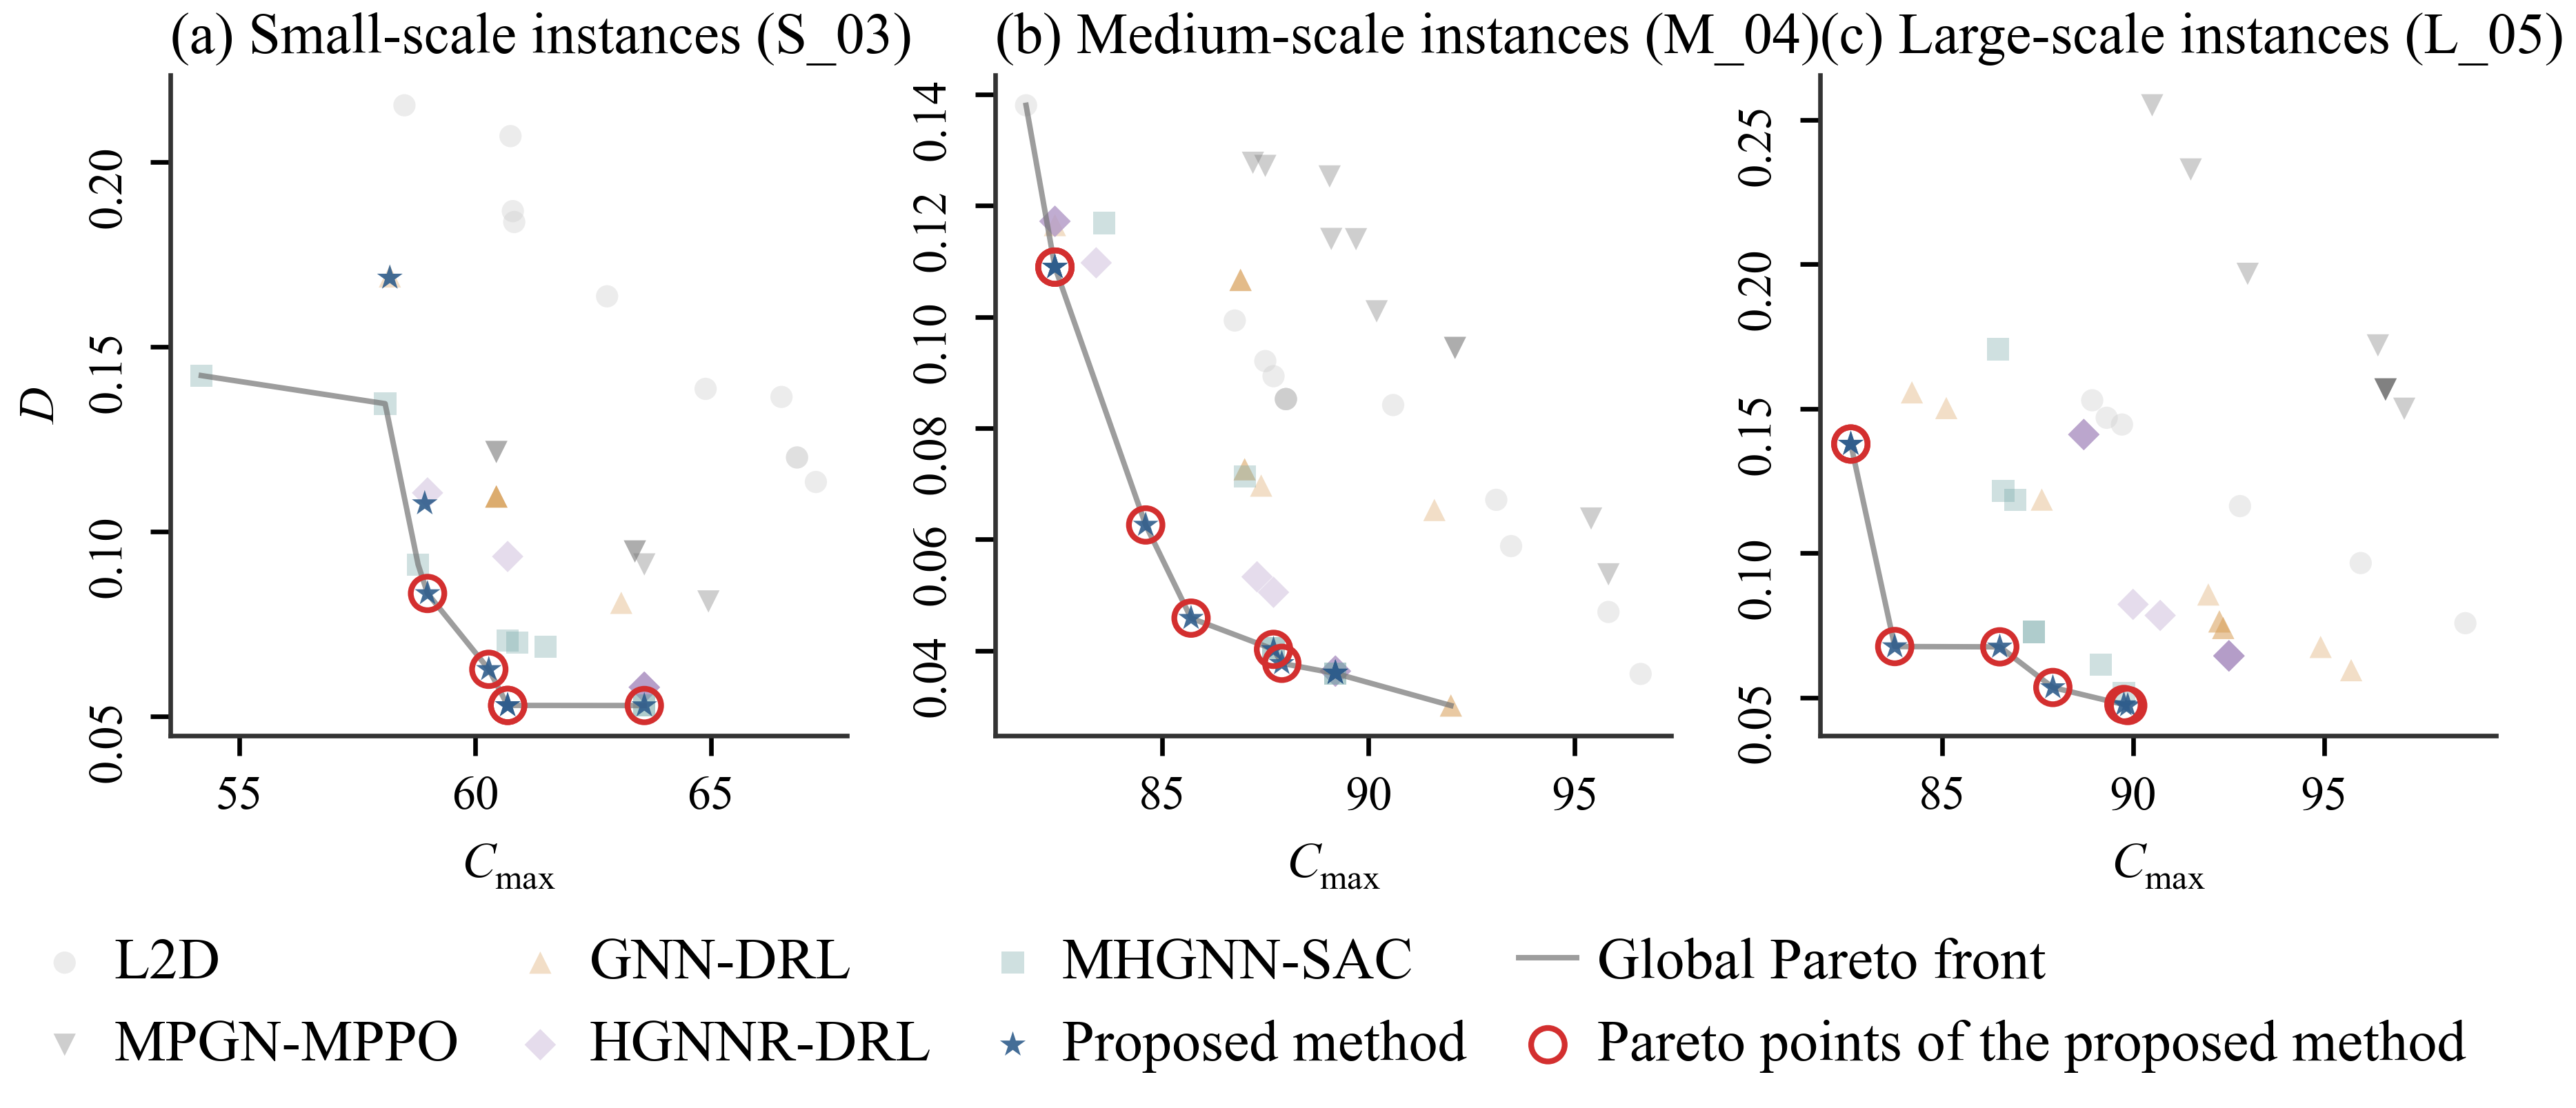
\includegraphics[width=0.85\linewidth]{figures/F9lyk强化学习泛化实验帕累托前沿图_新版候选_原图.png}
    \caption{Objective trade-offs on representative S03, M04, and L05 test instances.}
    \label{fig:pareto_front_unseen_scenarios}
\end{figure*}

Figure~\ref{fig:pareto_front_unseen_scenarios} illustrates the objective trade-offs on S03, M04,
and L05. Several HGNN-PPO solutions contribute to the pooled nondominated front on M04 and L05,
whose HV values are 1.131 and 1.195. On L05, the latter is approximately 10.6\% above the
MHGNN-SAC value of 1.080. Along these fronts, lower deviation can require longer completion time,
providing alternatives for different objective preferences. On S03, MHGNN-SAC has a stronger
short-makespan region and a higher HV, 1.134 versus 1.013. The proposed policy consequently
provides competitive trade-offs without covering every extreme of the objective space equally well.

% F9对应S03、M04、L05，按可见前沿与表格解释优点和失效边界。
% 图中的全局前沿仅为比较方法所得点的合并非支配前沿，不是已知真实最优前沿。

\begin{figure*}[!htbp]
    \centering
    \captionsetup{name=Figure}
    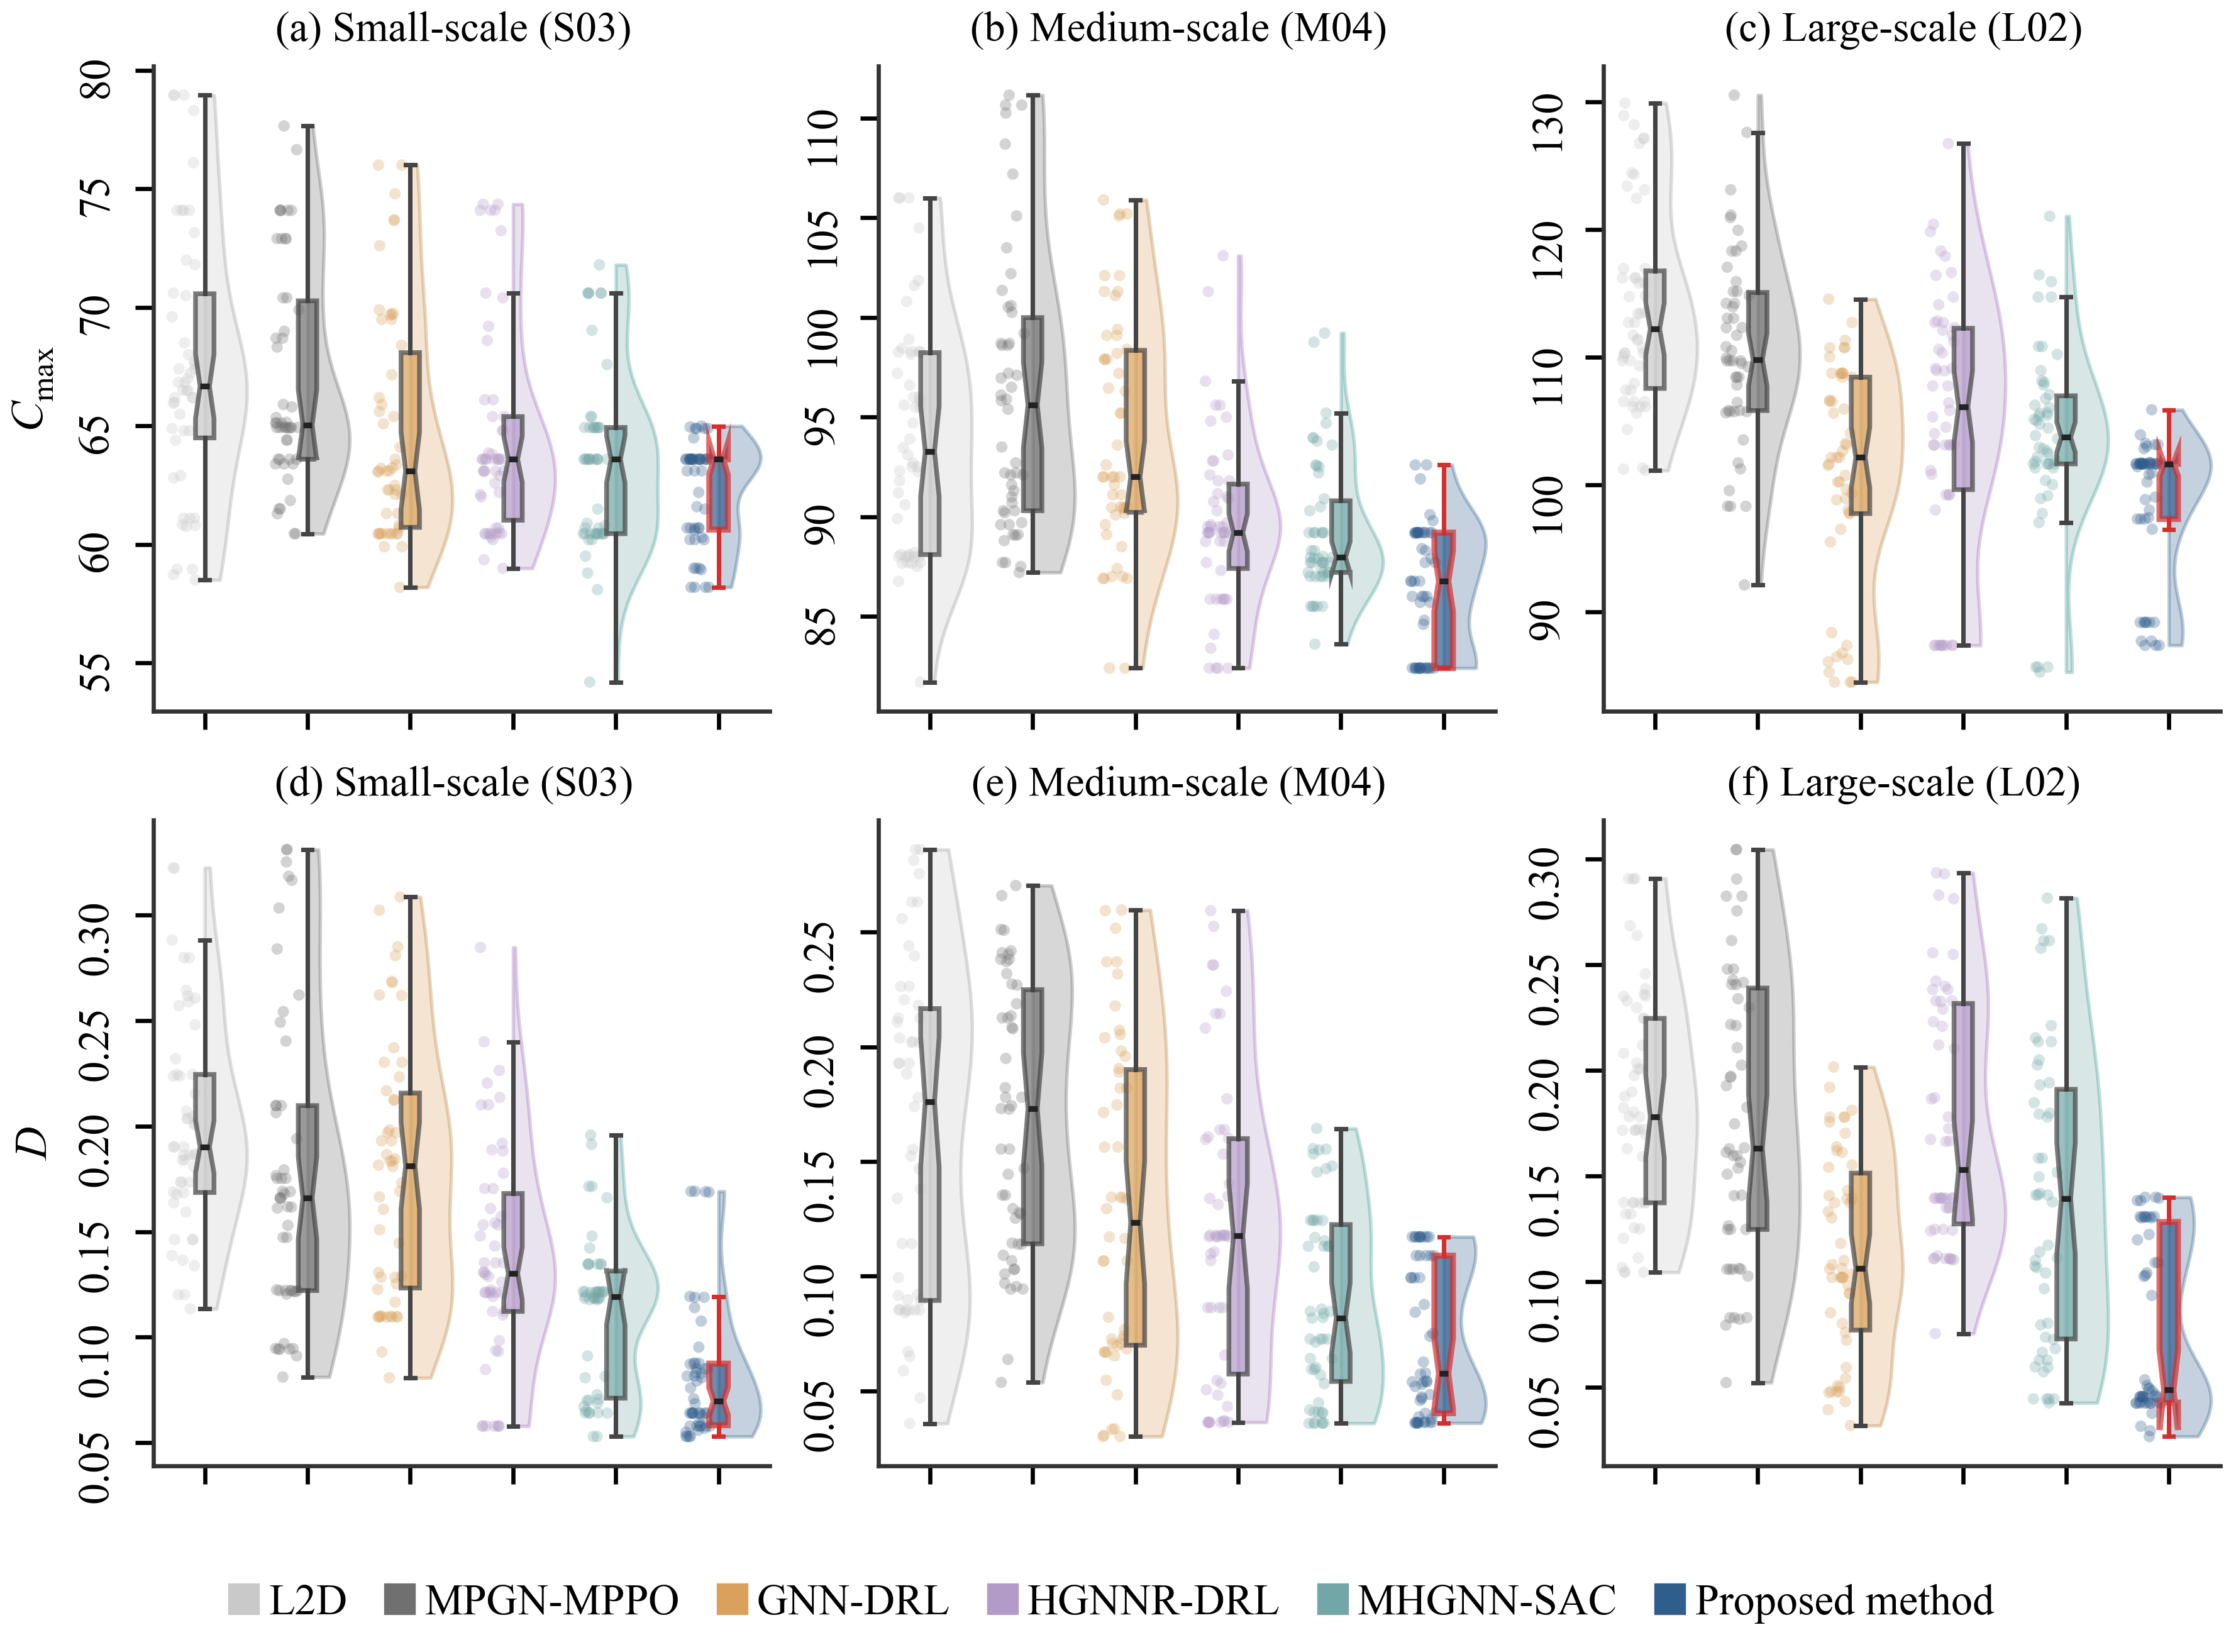
\includegraphics[width=0.85\linewidth]{figures/F10lyk六算法_S03_M04_L05_Cmax_Dt_箱线图_2列3行_原图.png}
    \caption{Objective-value distributions on representative S03, M04, and L02 test instances.}
    \label{fig:objective_distributions_test_scenarios}
\end{figure*}

The distribution plots in Fig.~\ref{fig:objective_distributions_test_scenarios} concern S03, M04,
and L02. HGNN-PPO places much of its deviation distribution in a lower region while maintaining
competitive makespan values. On L02, its HV is 1.060 compared with 1.026 for MHGNN-SAC, whereas
their Spread values, 0.927 and 0.932, are close. Here, the lower-deviation solutions do not imply
a large improvement in distribution uniformity. These examples connect the aggregate indicators
to the locations and ranges of the displayed objective values.

% F10实际面板为L02，文件名含L05不代表图内算例，图注和正文已按面板修正。
% TODO：图中样本量、点的含义、重复训练与重复评价的层次须从日志核实。
% TODO：现有泛化工作表含分布强化版名称，数据说明仅确认复制与数值校验，
% 不能据此认定原始实验可追溯；补齐场景、运行和计算脚本对应。

\subsection{Discussion}
\label{subsec:experimental_discussion}

The results provide complementary views of the state encoder. Parameter analysis identifies a common
configuration for the comparisons. Attention ablation shows lower late-training objective curves
for the complete configuration, particularly on the larger groups. The instance-wise tables show
that this advantage is more consistent for makespan than for deviation. Independent testing further
shows favorable average solution-set coverage, while individual cases reveal limits in extreme
trade-offs and distribution uniformity.

% 讨论按参数、消融、实例目标和独立解集四层证据归纳，不夸大逐例优势。

The mechanism is consistent with the need to distinguish technological, resource, and assembly
information before selecting a dispatching rule. Role-specific readout then exposes relevant
information to routing, sequencing, and recovery. However, the current attention comparison does not
separately identify every meta-path's effect, and the rule-selection display depends on the candidate
pool used to produce it. Improvements in a selector and improvements in its available rules must
therefore be distinguished when interpreting the method.

% 不将规则库质量提升归因于编码器，也不将一次整体消融解释为各路径因果作用。

The demonstrated scope is the supplied instance and disturbance configurations. Explicit urgent-order
evaluation requires a verified mapping between arrival scenarios and the reported test instances.
Likewise, real-time applicability requires measurements of graph updating, encoding, and rule decoding,
which are not established by objective quality alone. Repeated-run uncertainty, fully specified
normalization, and a documented baseline and rule pool are needed before extending these descriptive
comparisons to broader reliability or industrial-deployment claims.

% 已有图表不自动证明新增插单场景或现场实时性；缺失项保留明确核验接口。
% TODO：所有表格、模型版本、种子、训练偏好和完整日志需建立可追溯索引。
\FloatBarrier

\section{Conclusion and Future Work}
\label{sec:conclusion}

% 结论

% 总结本文研究工作，包括研究问题、提出的方法以及主要实验验证结果。
% 不应简单重复摘要内容，而应从研究目标、方法贡献和实验发现三个方面
% 对全文进行归纳总结。
%
% 所有关于算法性能提升、有效性或优势的描述，
% 都必须能够在第5章实验结果中找到对应的实验依据。
% 避免在结论中加入未经实验验证的泛化性结论。
%
% 最后一部分应结合本文提出的局限性，
% 给出具有针对性的未来研究方向，
% 而不是简单罗列宽泛的未来工作。

\section*{Acknowledgements}
% List funding, institutional, technical, and other non-author contributions.

\section*{CRediT Authorship Contribution Statement}
% Assign applicable CRediT roles to every author.

\section*{Declaration of Competing Interest}
% Use the target journal's required declaration after confirming it is accurate.

\section*{Data Availability}
% State where data/code can be accessed, or explain justified access restrictions.

\section*{Declaration of Generative AI and AI-assisted Technologies}
% Include only if required, following the target journal's current policy.


% Remove this demonstration command after adding verified citations in the text.
\nocite{schulman2017ppo}
\bibliographystyle{elsarticle-num}
\bibliography{references/references}

\end{document}
